
%%%----------------------------------------------------------
%%%----------------------------------------------------------
%%%----------------------------------------------------------
%%%----------------------------------------------------------
%%%----------------------------------------------------------
\chapter{Stairs}
%%%----------------------------------------------------------

The activity "stairs" will be analyzed here with graphics.
%%%----------------------------------------------------------
\section{Test case 1}
%%%----------------------------------------------------------
Test case 1 in Fig.~\ref{fig:Test_case_stairs_1}
\begin{figure}
	\centering\small
	\setlength{\tabcolsep}{0mm}	% alle Spaltenränder auf 0mm
	\begin{tabular}{c@{\hspace{12mm}}c} % mittlerer Abstand = 12mm
		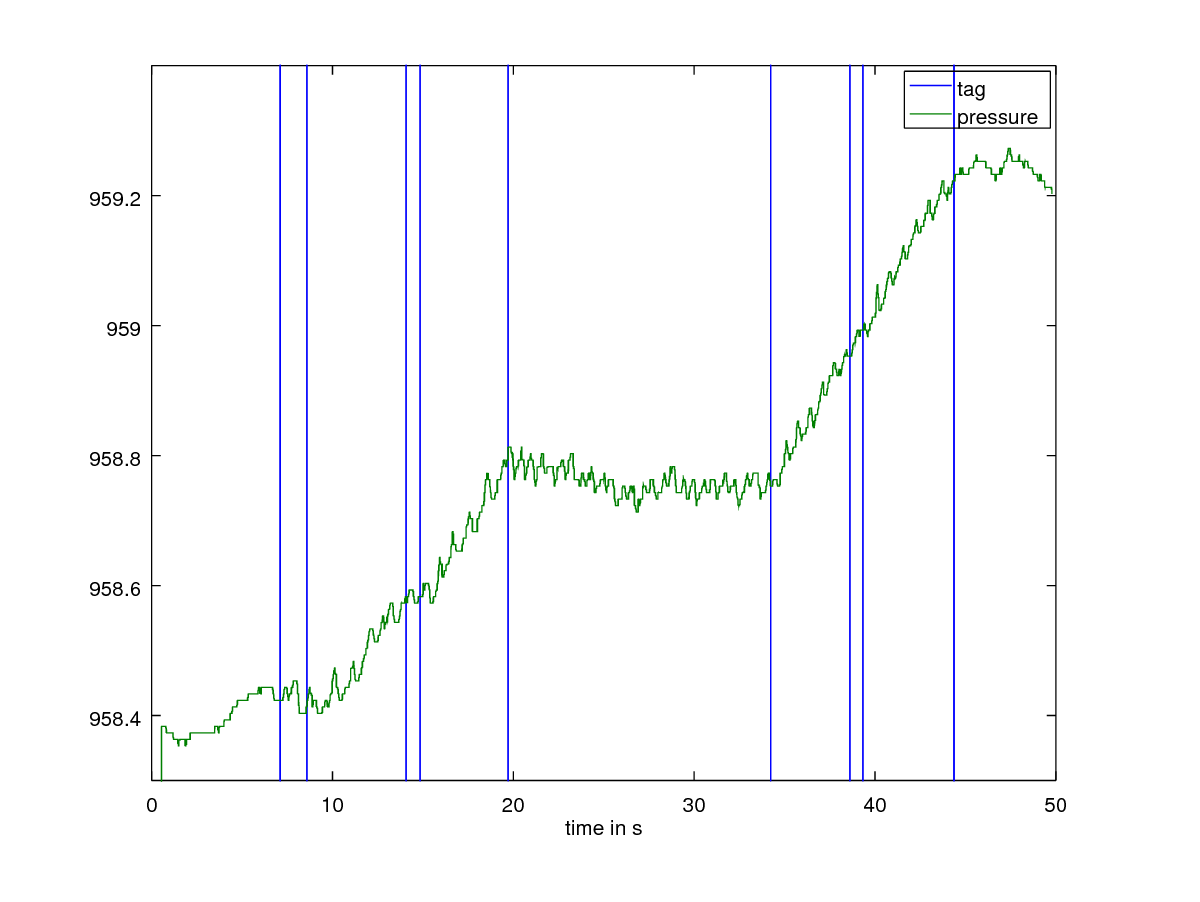
\includegraphics[width=.45\textwidth]{stairsfhdown_p} &
		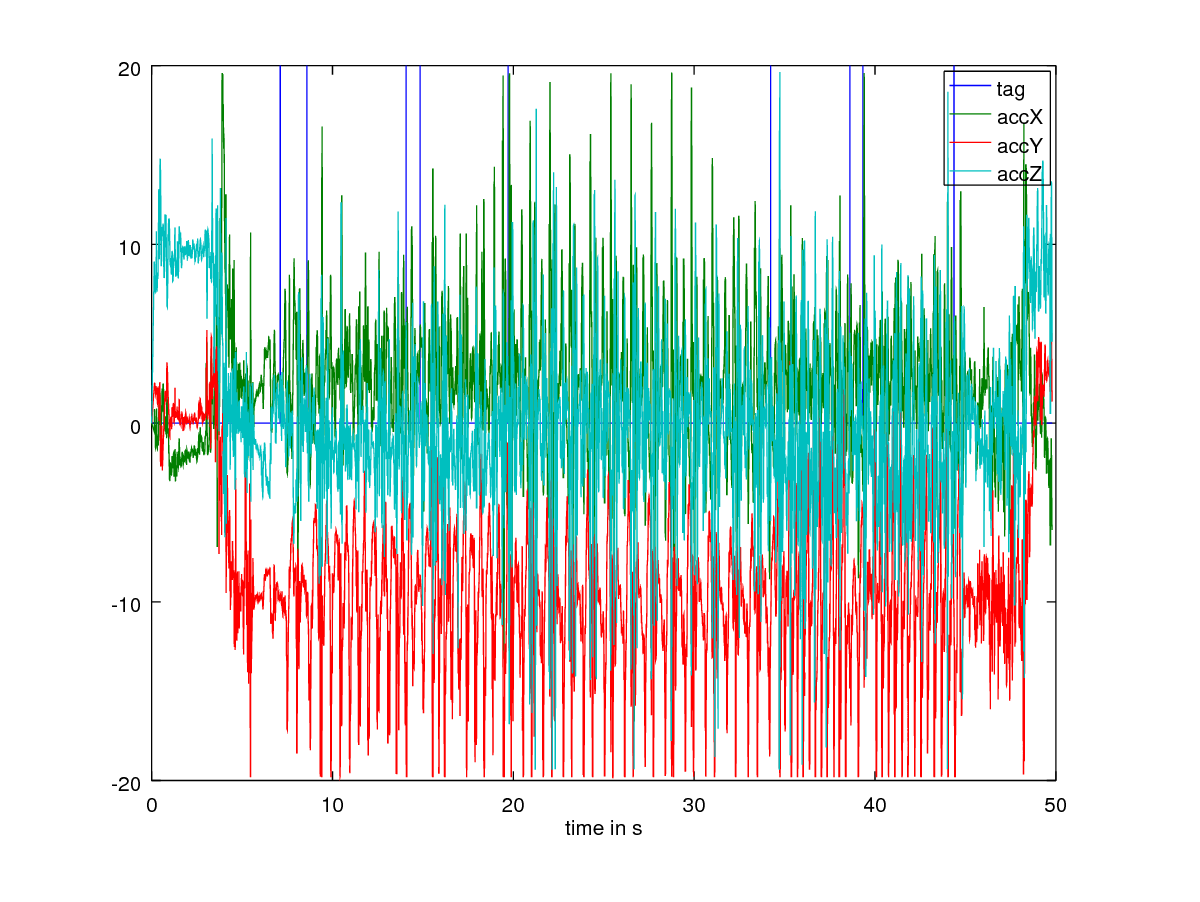
\includegraphics[width=.45\textwidth]{stairsfhdown_a} 
		\\
		(a) & (b)
		\\[4pt]	%vertical extra spacing (4 points)
		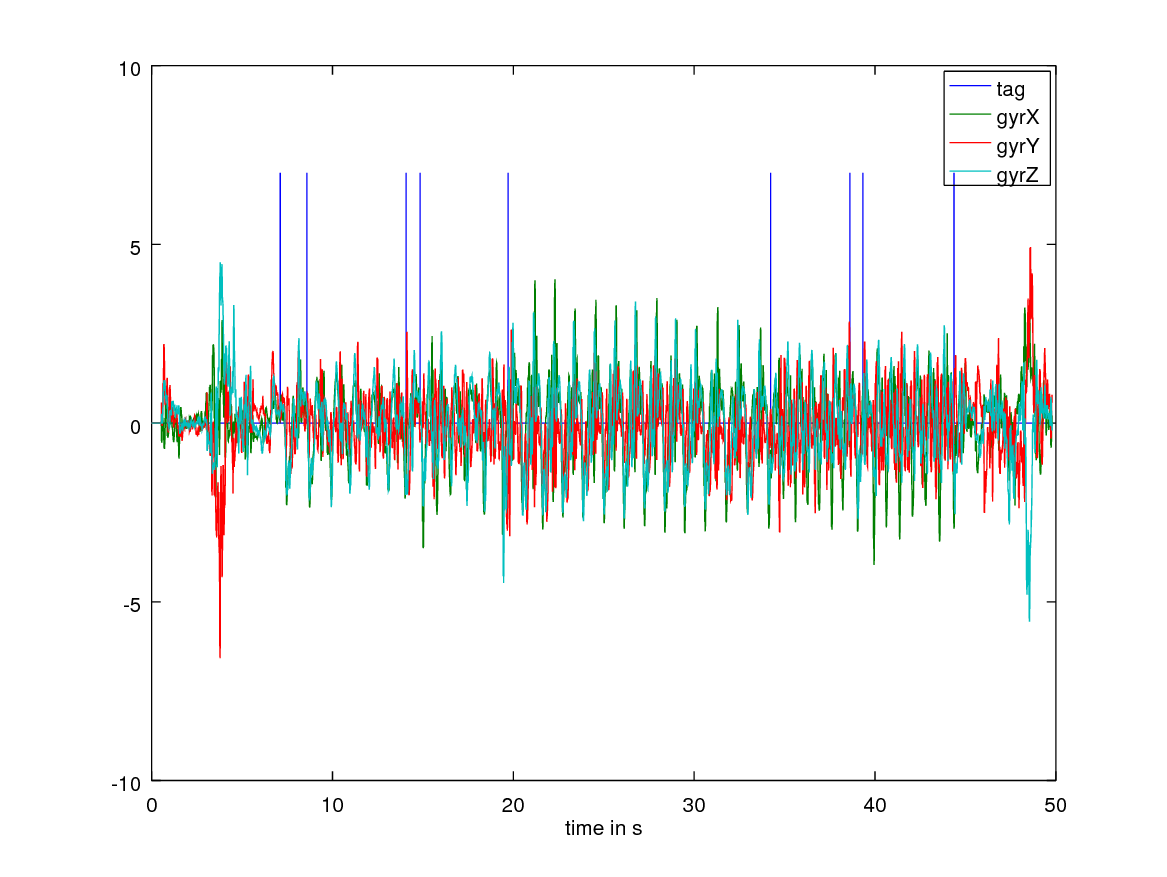
\includegraphics[width=.45\textwidth]{stairsfhdown_g} &
		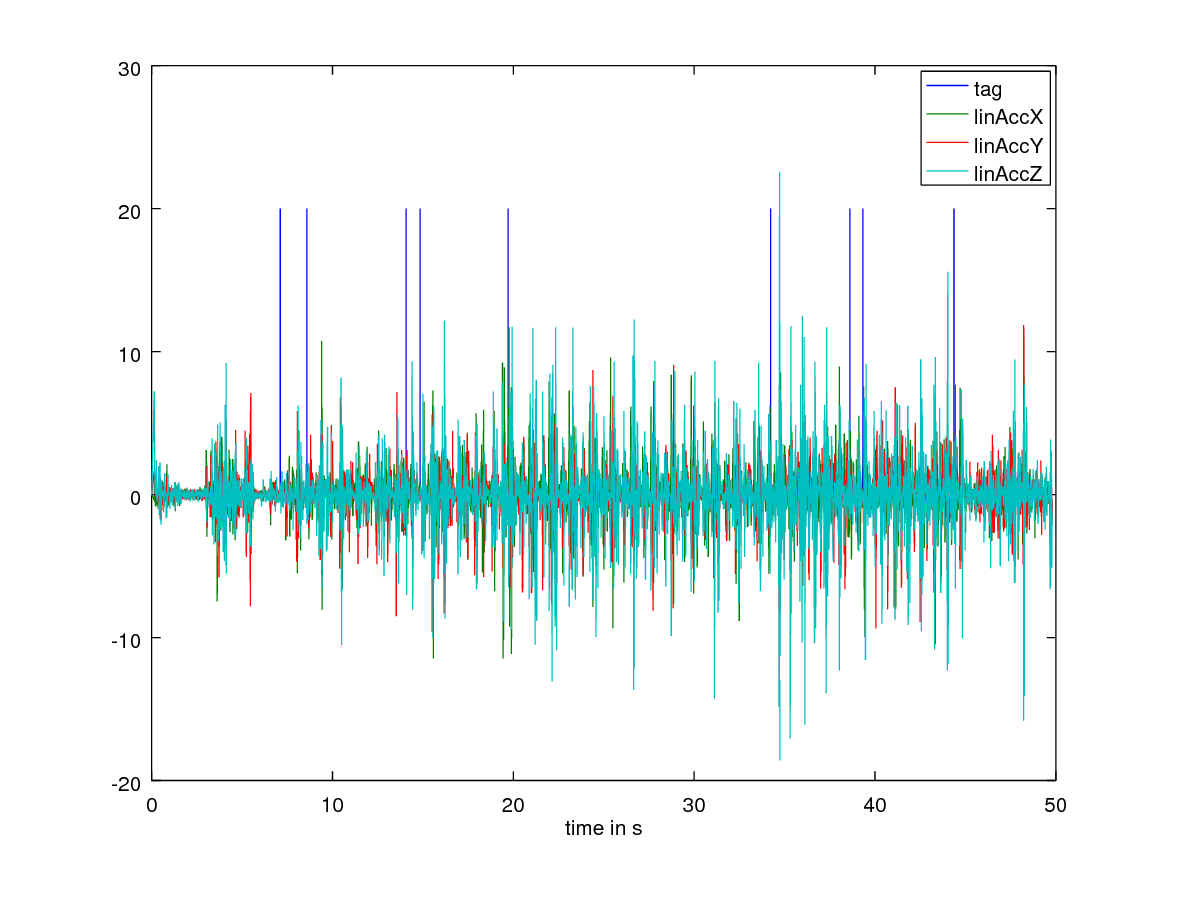
\includegraphics[width=.45\textwidth]{stairsfhdown_la} 
		\\
		(c) & (d)
		\\[4pt]	%vertical extra spacing (4 points)
		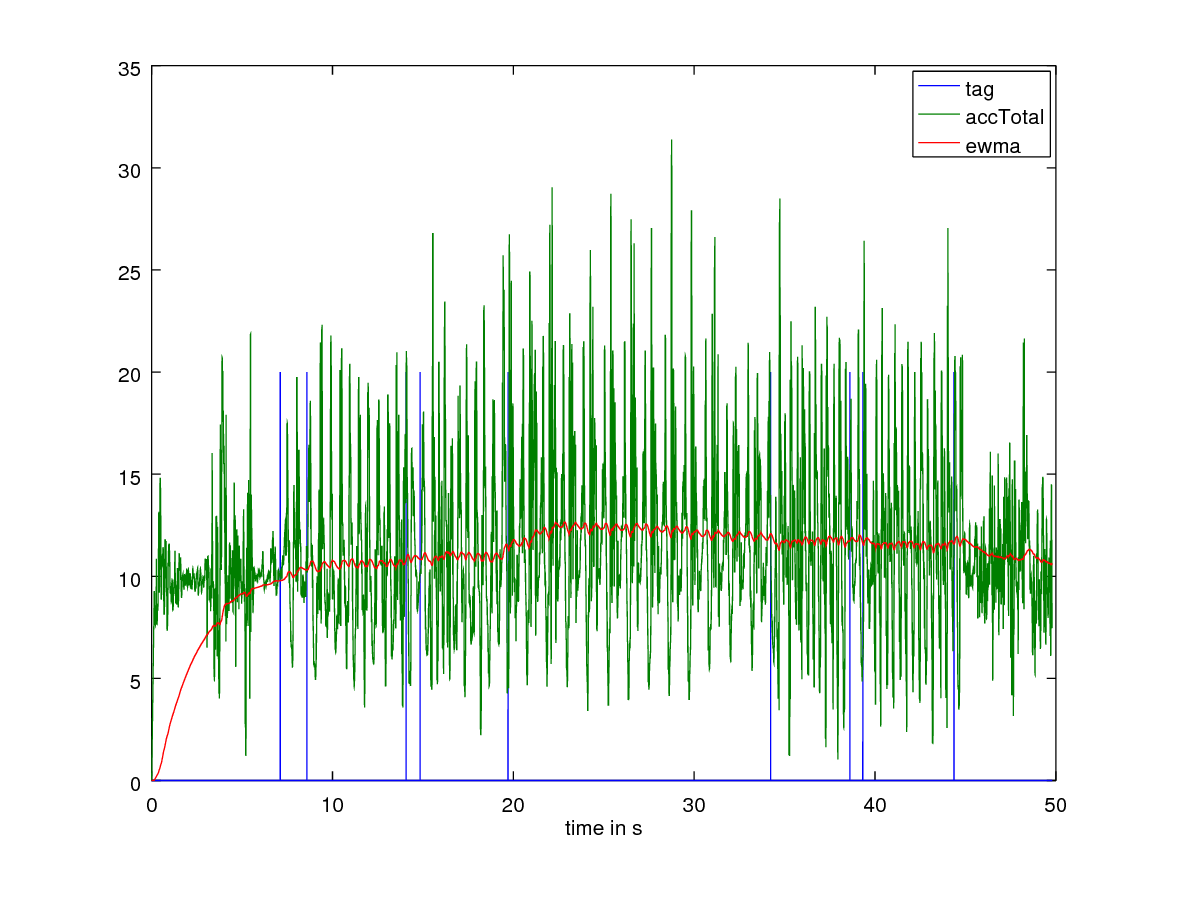
\includegraphics[width=.45\textwidth]{stairsfhdown_atotal} &
		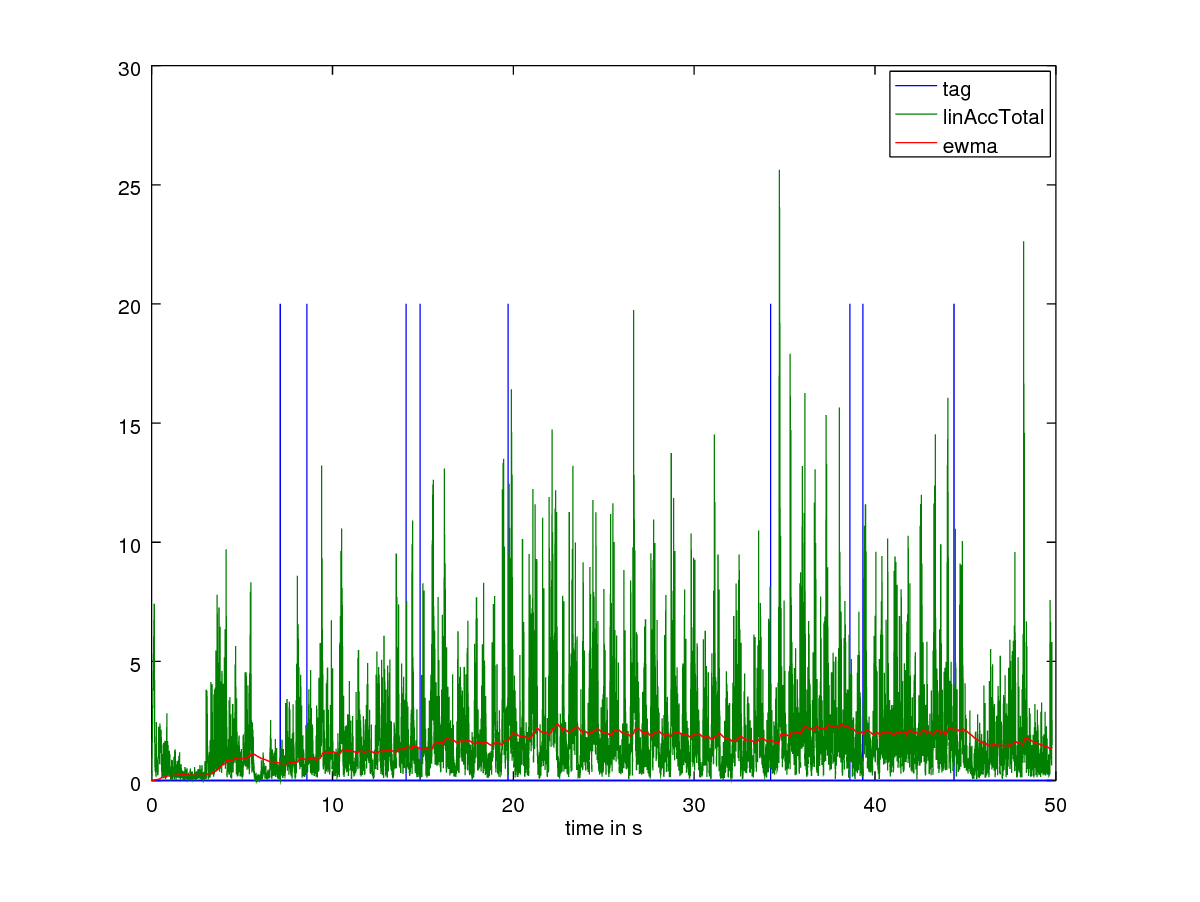
\includegraphics[width=.45\textwidth]{stairsfhdown_latotal} 
		\\
		(e) & (f)
	\end{tabular}
	%
	\caption{Test case 1}
	\label{fig:Test_case_stairs_1}
\end{figure}

%%%----------------------------------------------------------
\section{Test case 2}
%%%----------------------------------------------------------

Test case 2 in Fig.~\ref{fig:Test_case_stairs_2}
\begin{figure}
	\centering\small
	\setlength{\tabcolsep}{0mm}	% alle Spaltenränder auf 0mm
	\begin{tabular}{c@{\hspace{12mm}}c} % mittlerer Abstand = 12mm
		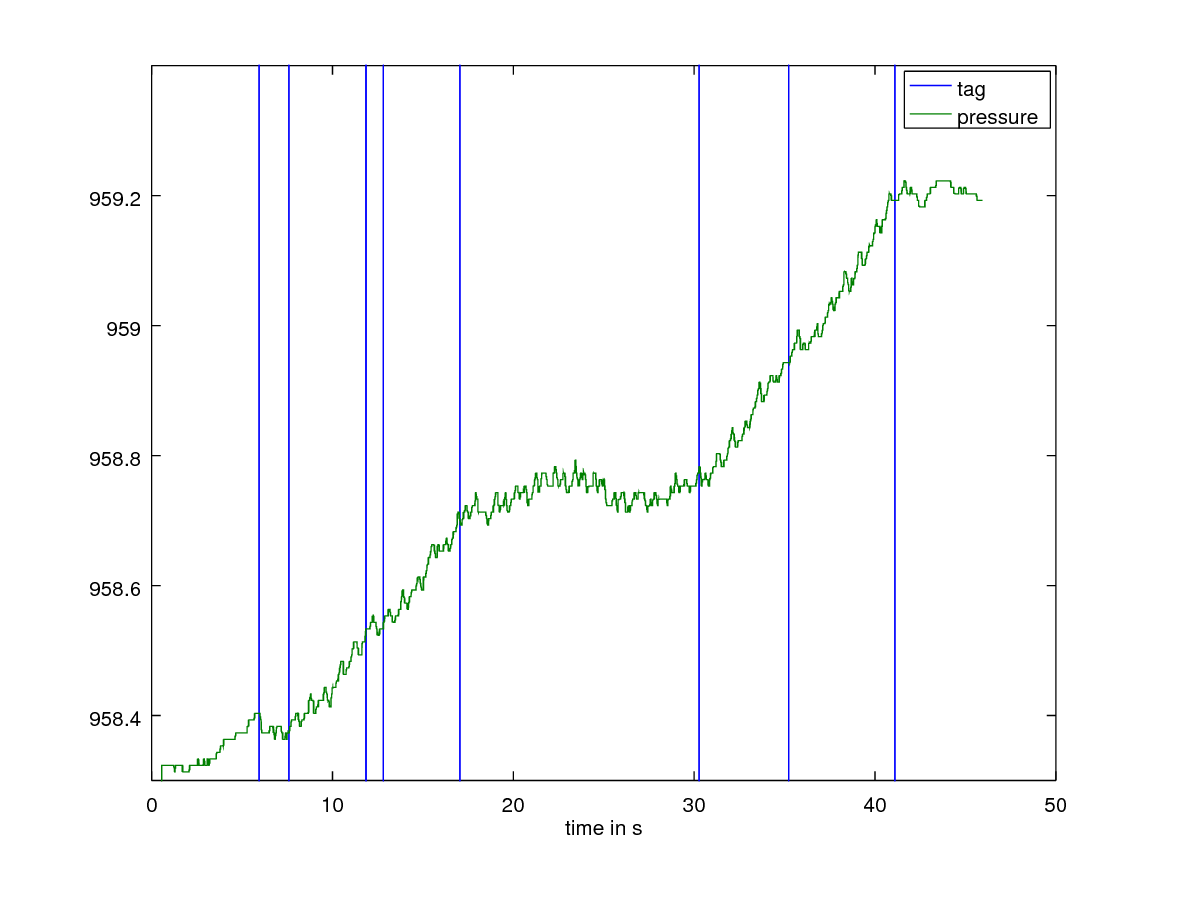
\includegraphics[width=.45\textwidth]{stairsfhdown2_p} &
		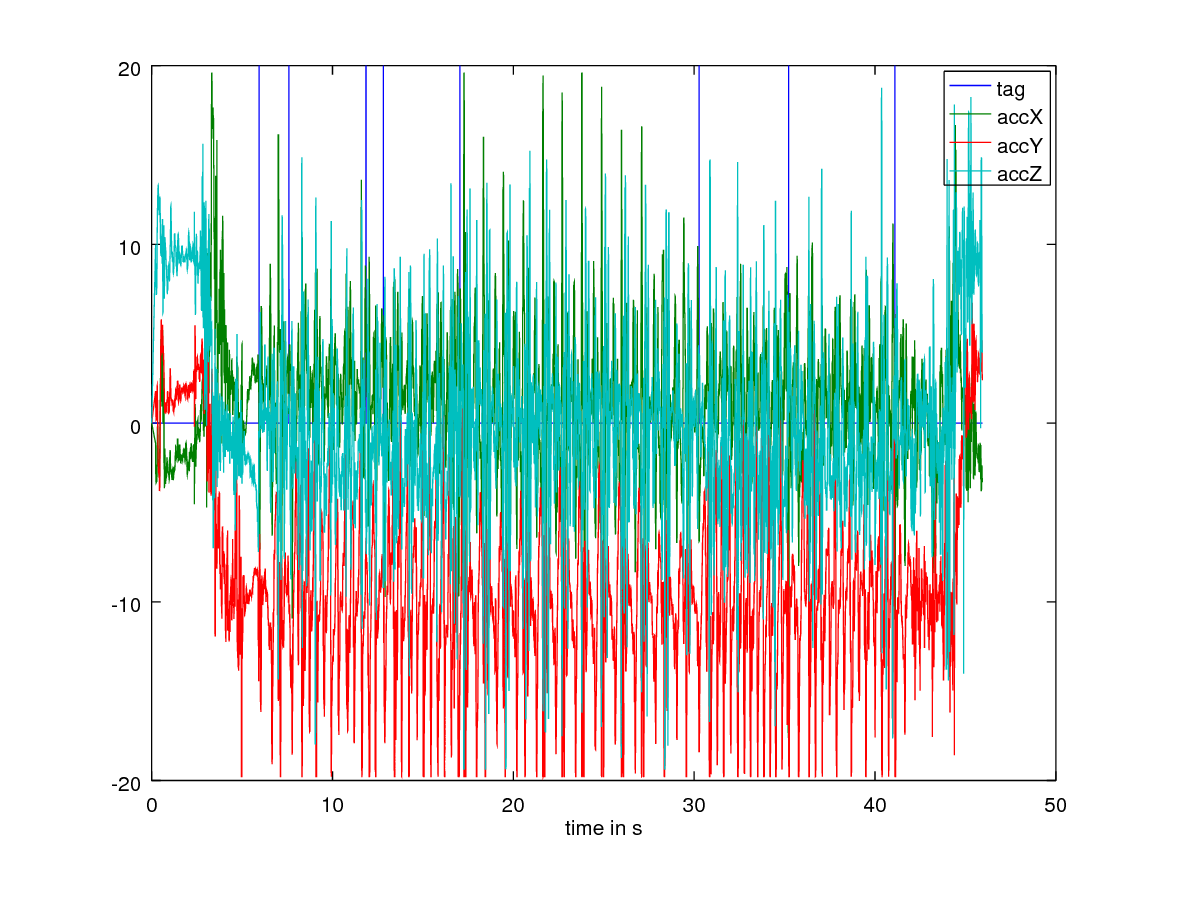
\includegraphics[width=.45\textwidth]{stairsfhdown2_a} 
		\\
		(a) & (b)
		\\[4pt]	%vertical extra spacing (4 points)
		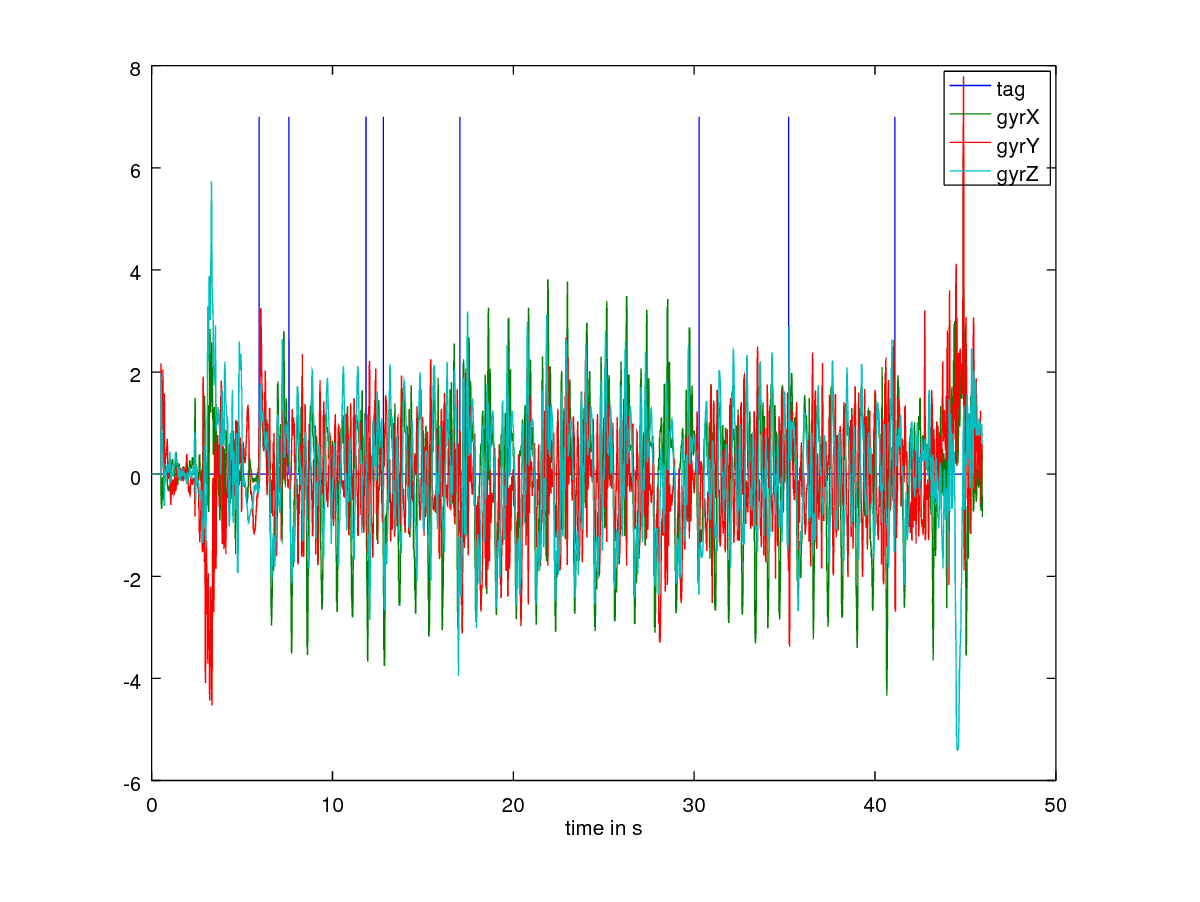
\includegraphics[width=.45\textwidth]{stairsfhdown2_g} &
		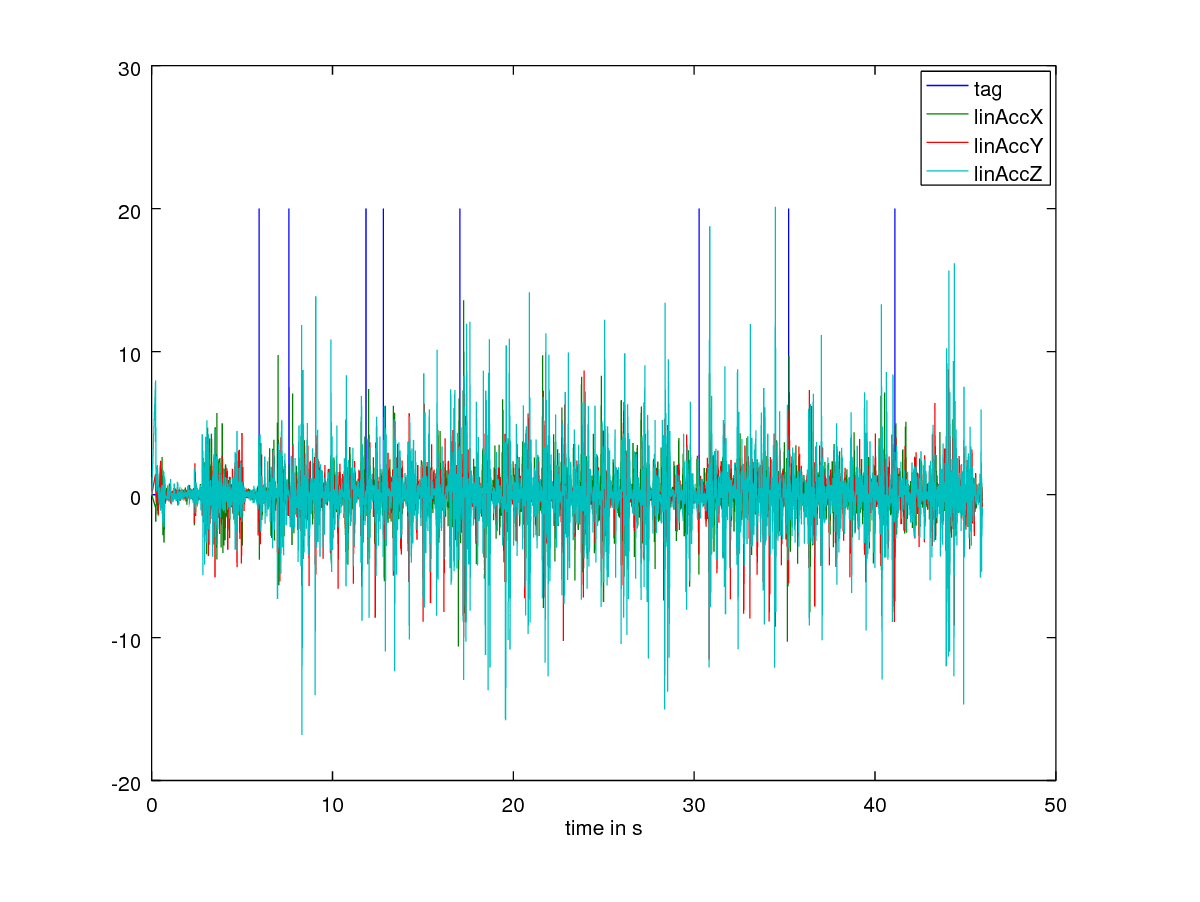
\includegraphics[width=.45\textwidth]{stairsfhdown2_la} 
		\\
		(c) & (d)
		\\[4pt]	%vertical extra spacing (4 points)
		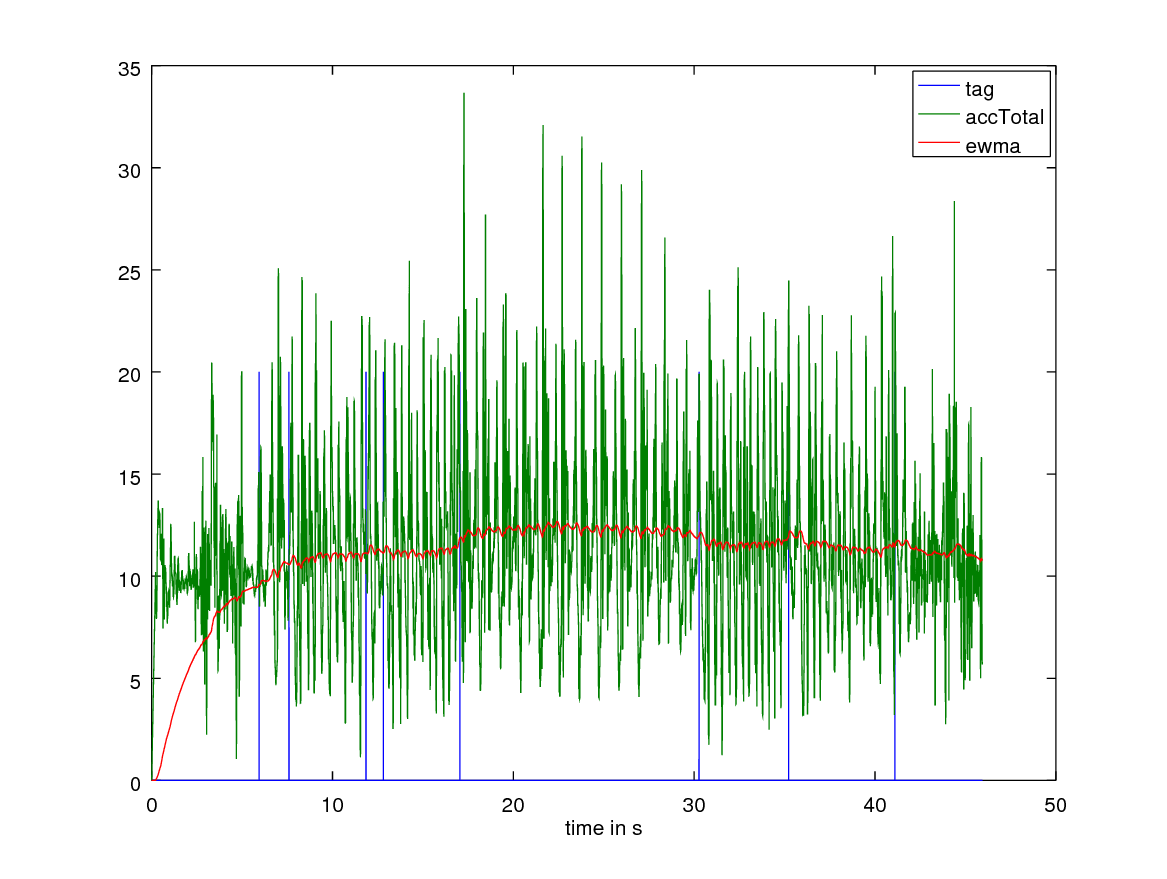
\includegraphics[width=.45\textwidth]{stairsfhdown2_atotal} &
		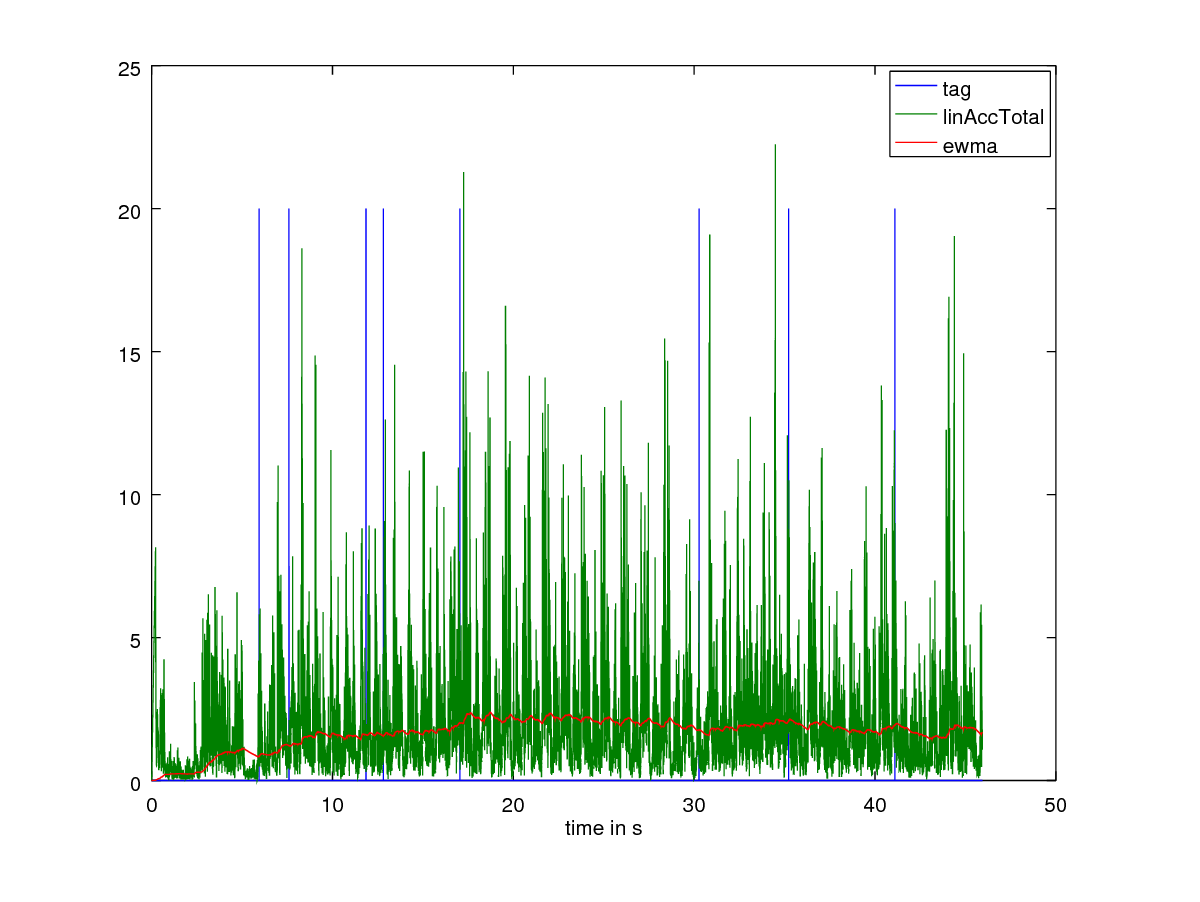
\includegraphics[width=.45\textwidth]{stairsfhdown2_latotal} 
		\\
		(e) & (f)
	\end{tabular}
	%
	\caption{Test case 2}
	\label{fig:Test_case_stairs_2}
\end{figure}


%%%----------------------------------------------------------
\section{Test case 3}
%%%----------------------------------------------------------
Test case 3 in Fig.~\ref{fig:Test_case_stairs_3}
\begin{figure}
	\centering\small
	\setlength{\tabcolsep}{0mm}	% alle Spaltenränder auf 0mm
	\begin{tabular}{c@{\hspace{12mm}}c} % mittlerer Abstand = 12mm
		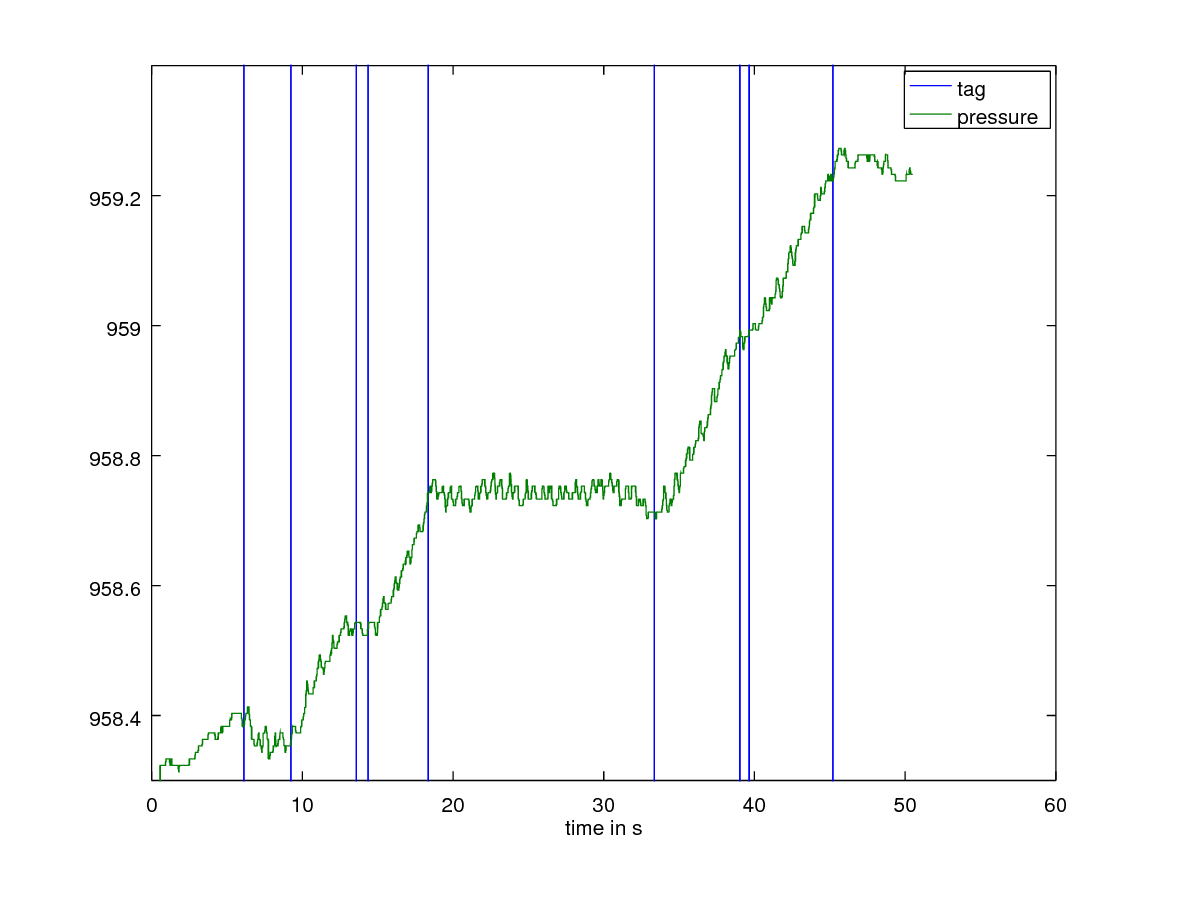
\includegraphics[width=.45\textwidth]{stairsfhdown6_p} &
		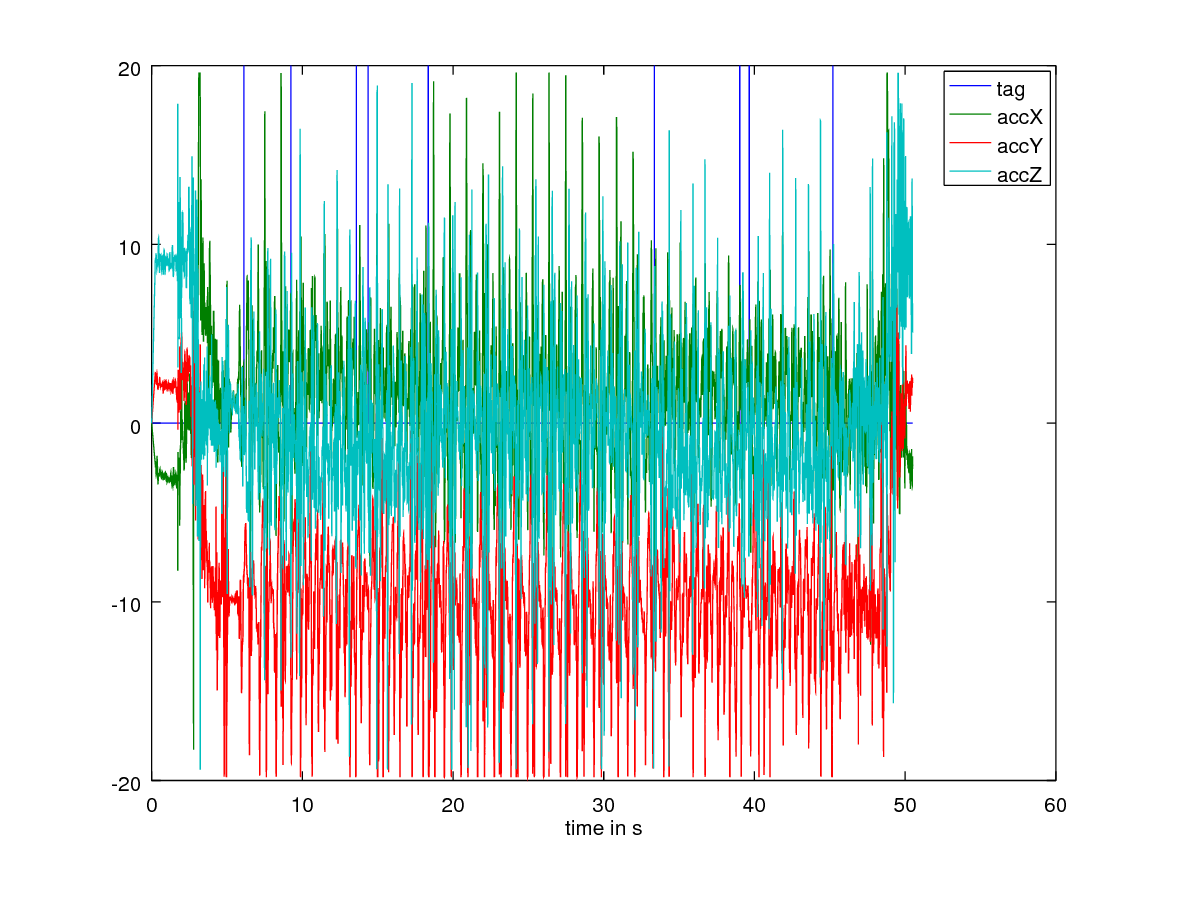
\includegraphics[width=.45\textwidth]{stairsfhdown6_a} 
		\\
		(a) & (b)
		\\[4pt]	%vertical extra spacing (4 points)
		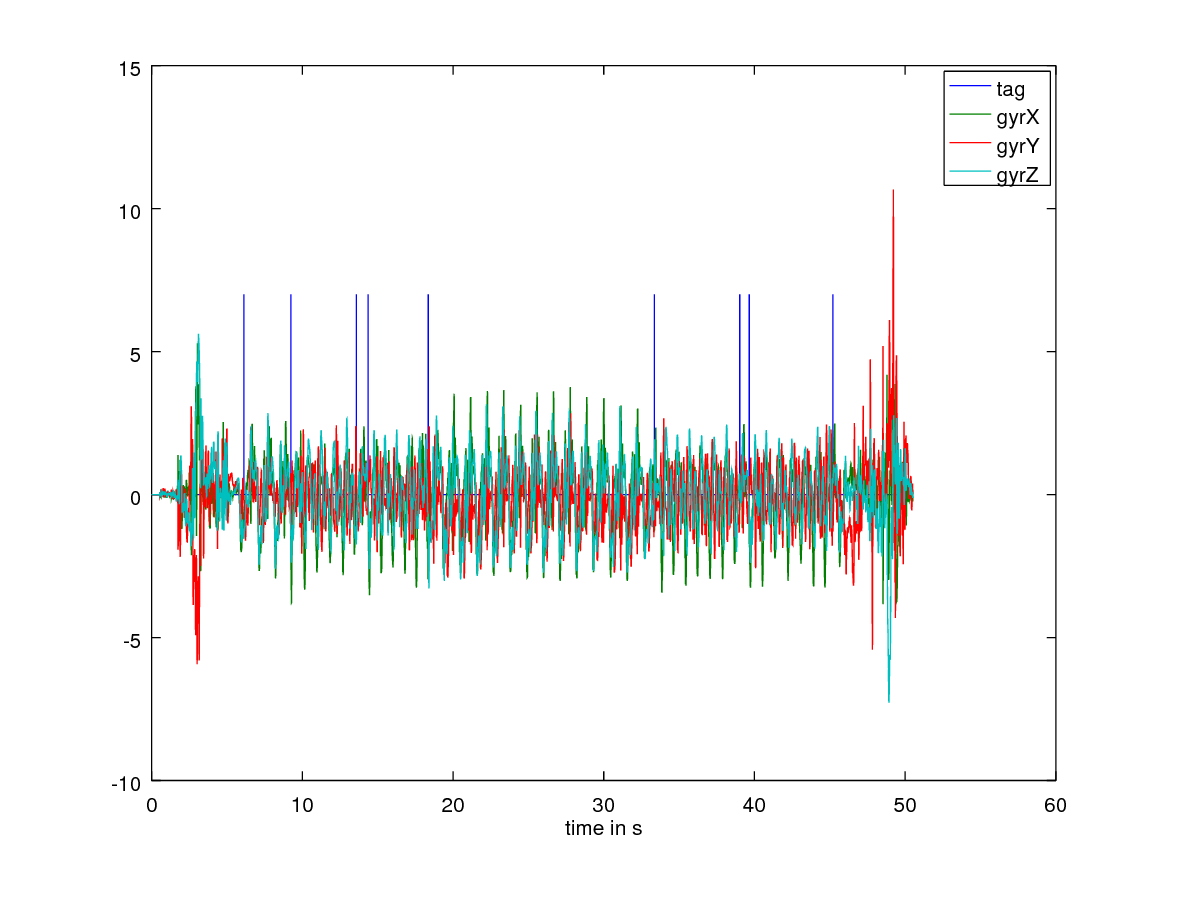
\includegraphics[width=.45\textwidth]{stairsfhdown6_g} &
		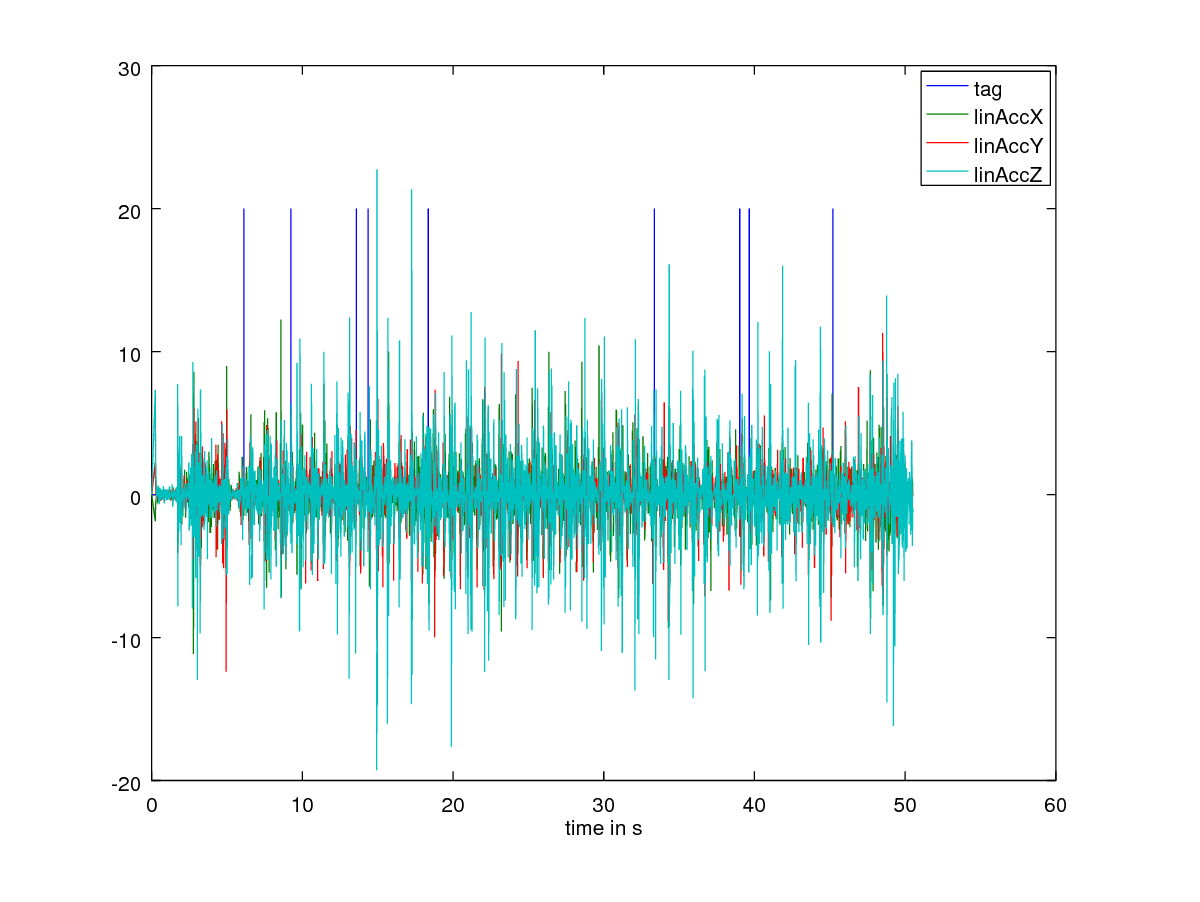
\includegraphics[width=.45\textwidth]{stairsfhdown6_la} 
		\\
		(c) & (d)
		\\[4pt]	%vertical extra spacing (4 points)
		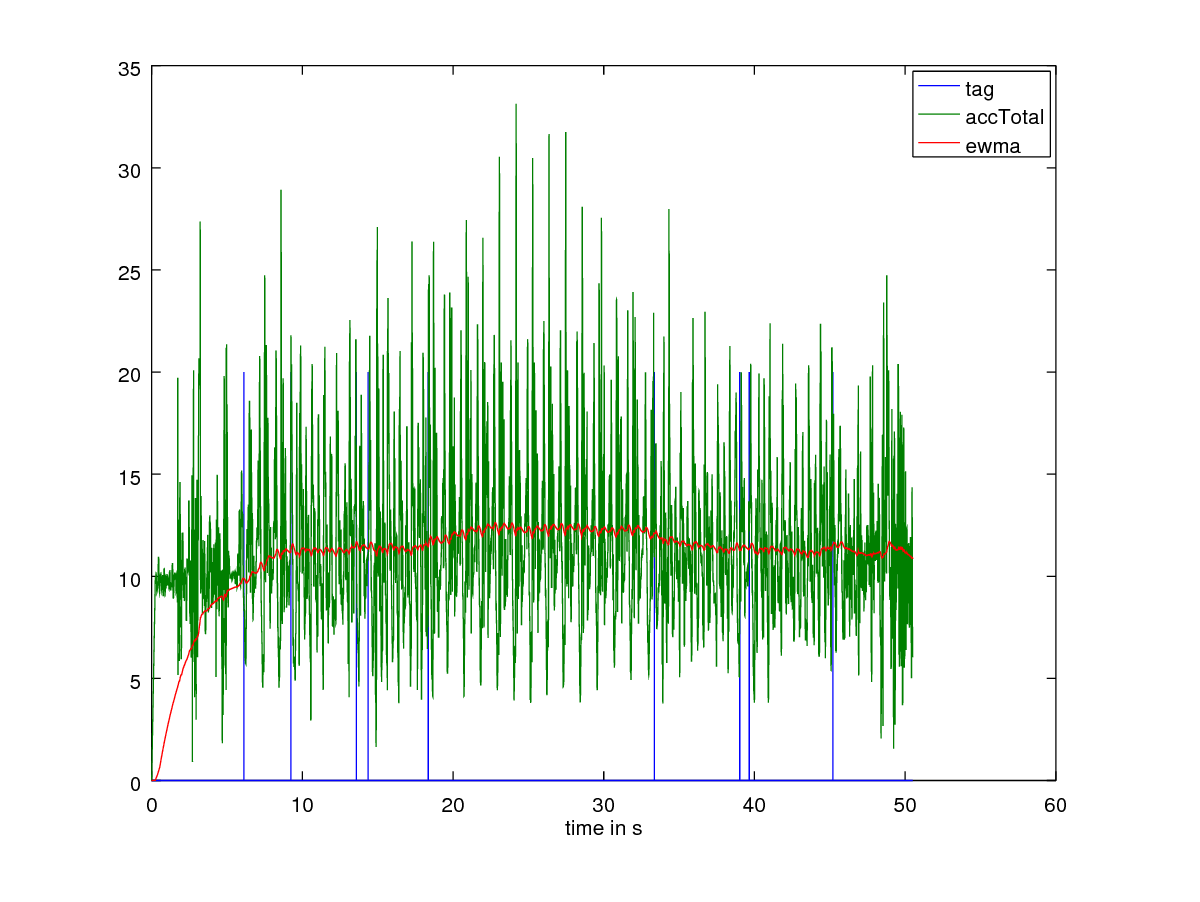
\includegraphics[width=.45\textwidth]{stairsfhdown6_atotal} &
		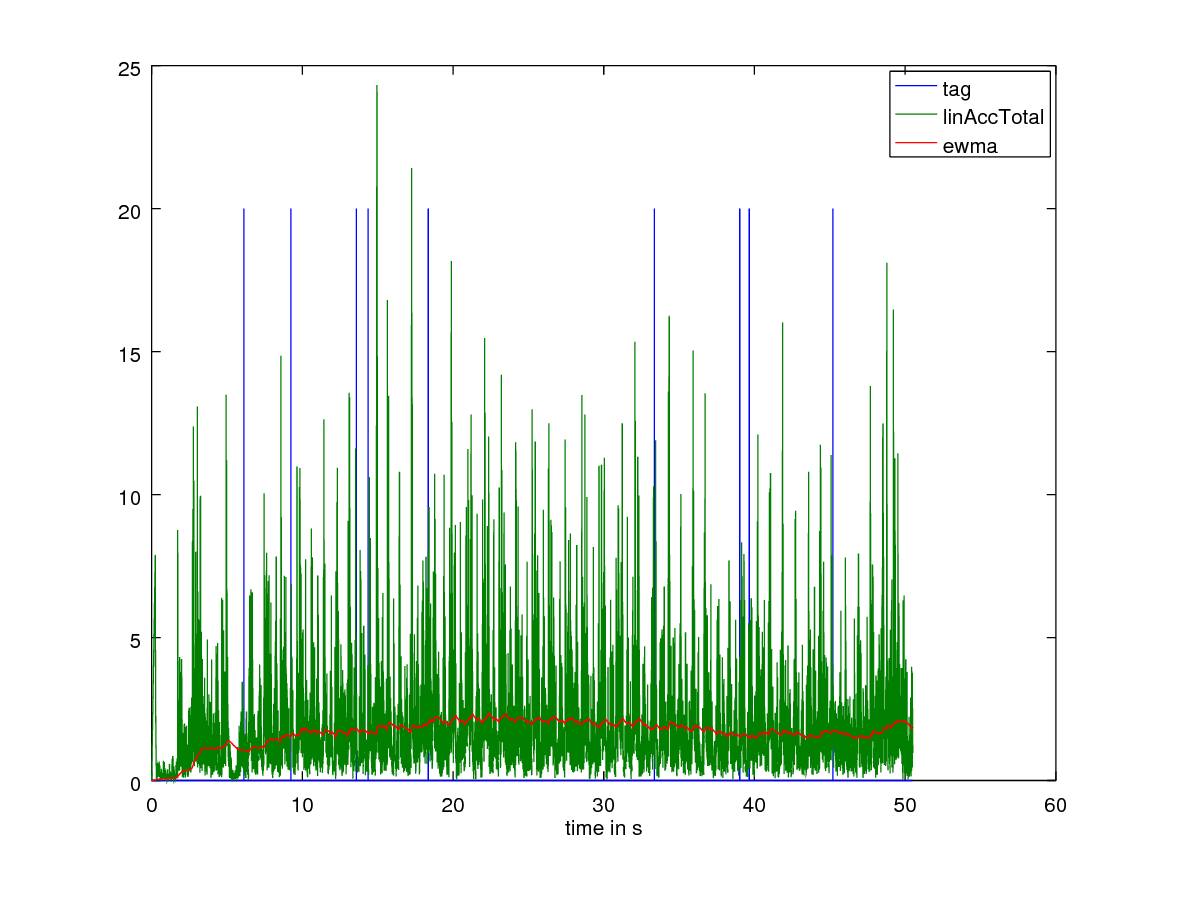
\includegraphics[width=.45\textwidth]{stairsfhdown6_latotal} 
		\\
		(e) & (f)
	\end{tabular}
	%
	\caption{Test case 3}
	\label{fig:Test_case_stairs_3}
\end{figure}

%%%----------------------------------------------------------
\section{Test case 4}
%%%----------------------------------------------------------
Test case 4 in Fig.~\ref{fig:Test_case_stairs_4}
\begin{figure}
	\centering\small
	\setlength{\tabcolsep}{0mm}	% alle Spaltenränder auf 0mm
	\begin{tabular}{c@{\hspace{12mm}}c} % mittlerer Abstand = 12mm
		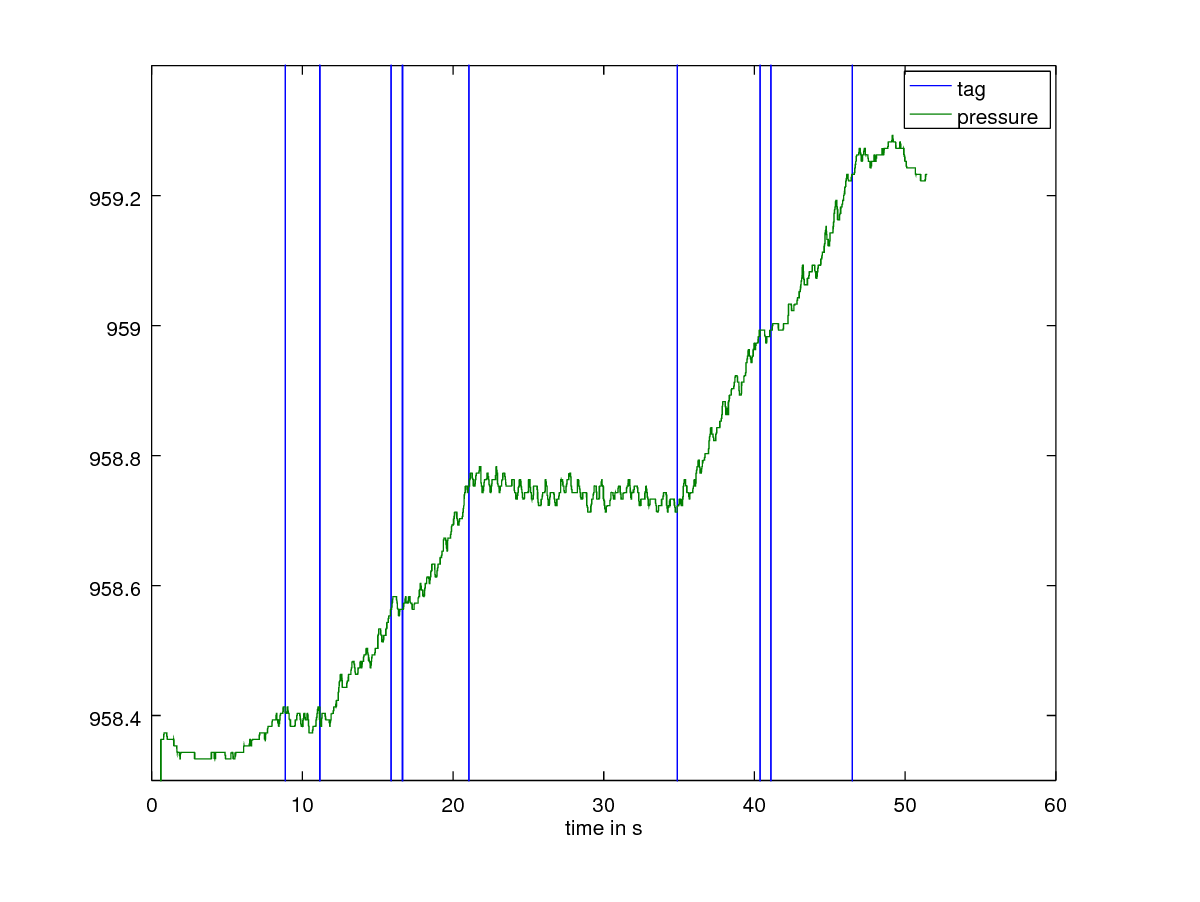
\includegraphics[width=.45\textwidth]{stairsfhdown10_p} &
		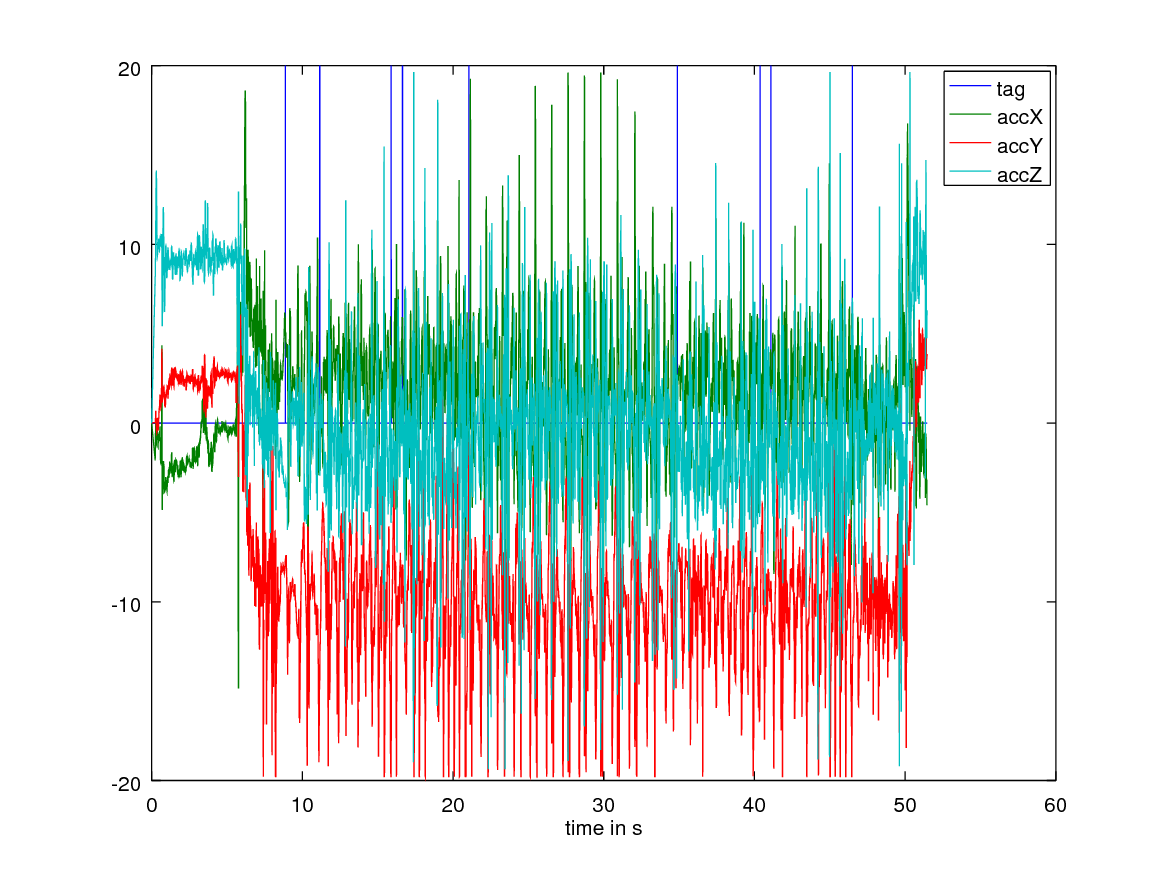
\includegraphics[width=.45\textwidth]{stairsfhdown10_a} 
		\\
		(a) & (b)
		\\[4pt]	%vertical extra spacing (4 points)
		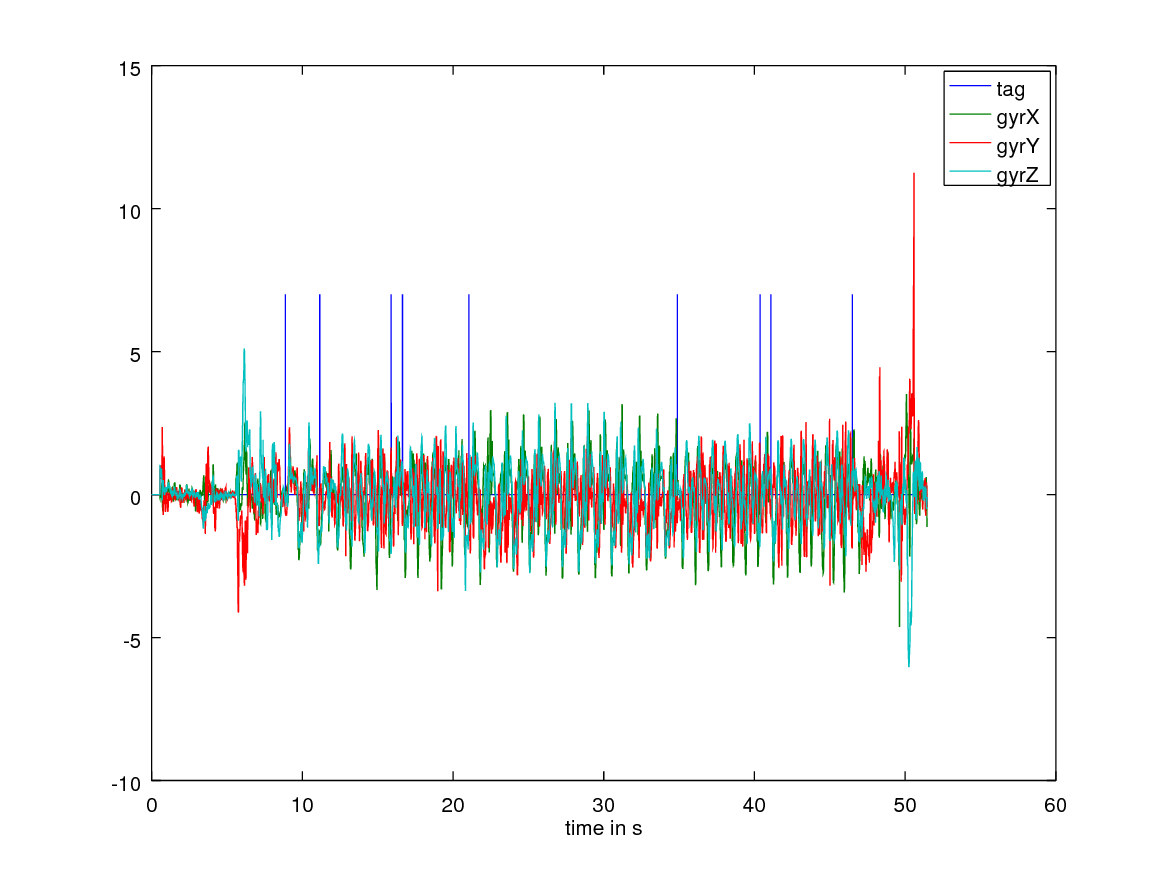
\includegraphics[width=.45\textwidth]{stairsfhdown10_g} &
		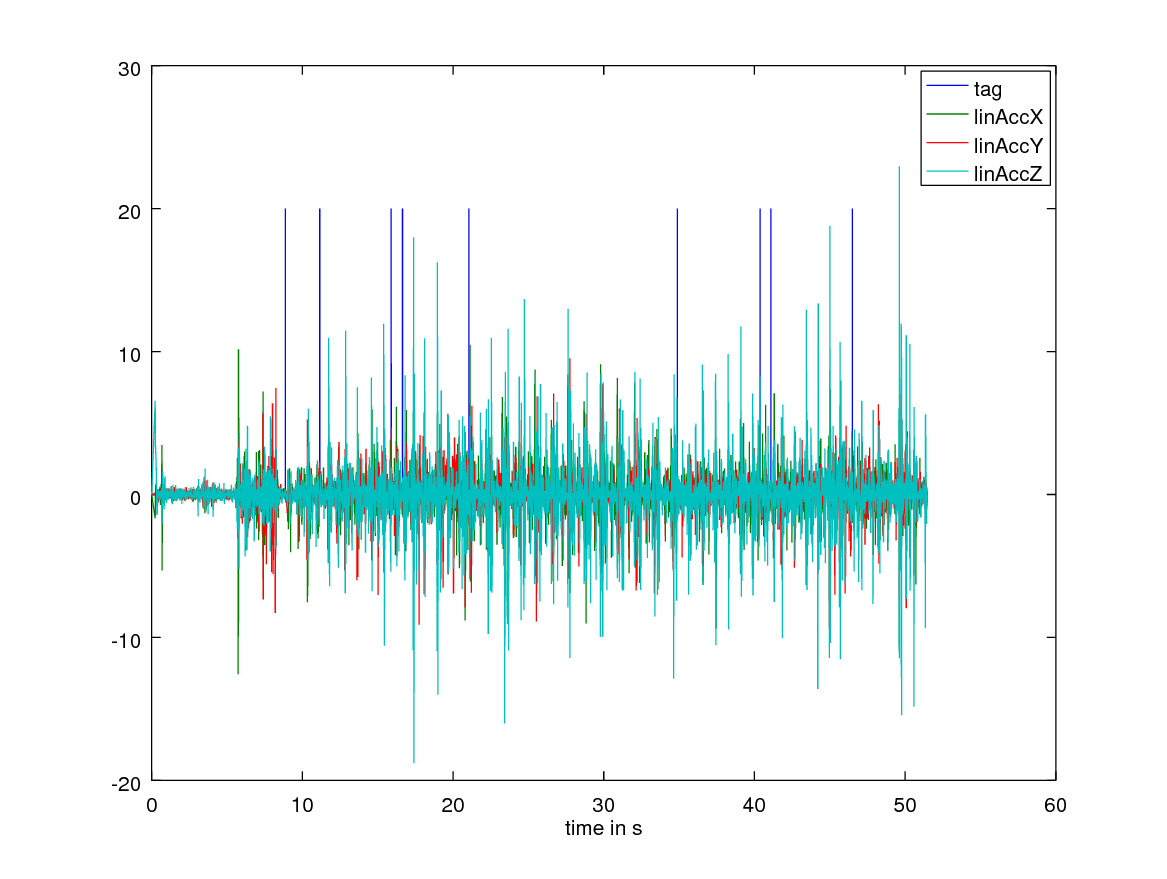
\includegraphics[width=.45\textwidth]{stairsfhdown10_la} 
		\\
		(c) & (d)
		\\[4pt]	%vertical extra spacing (4 points)
		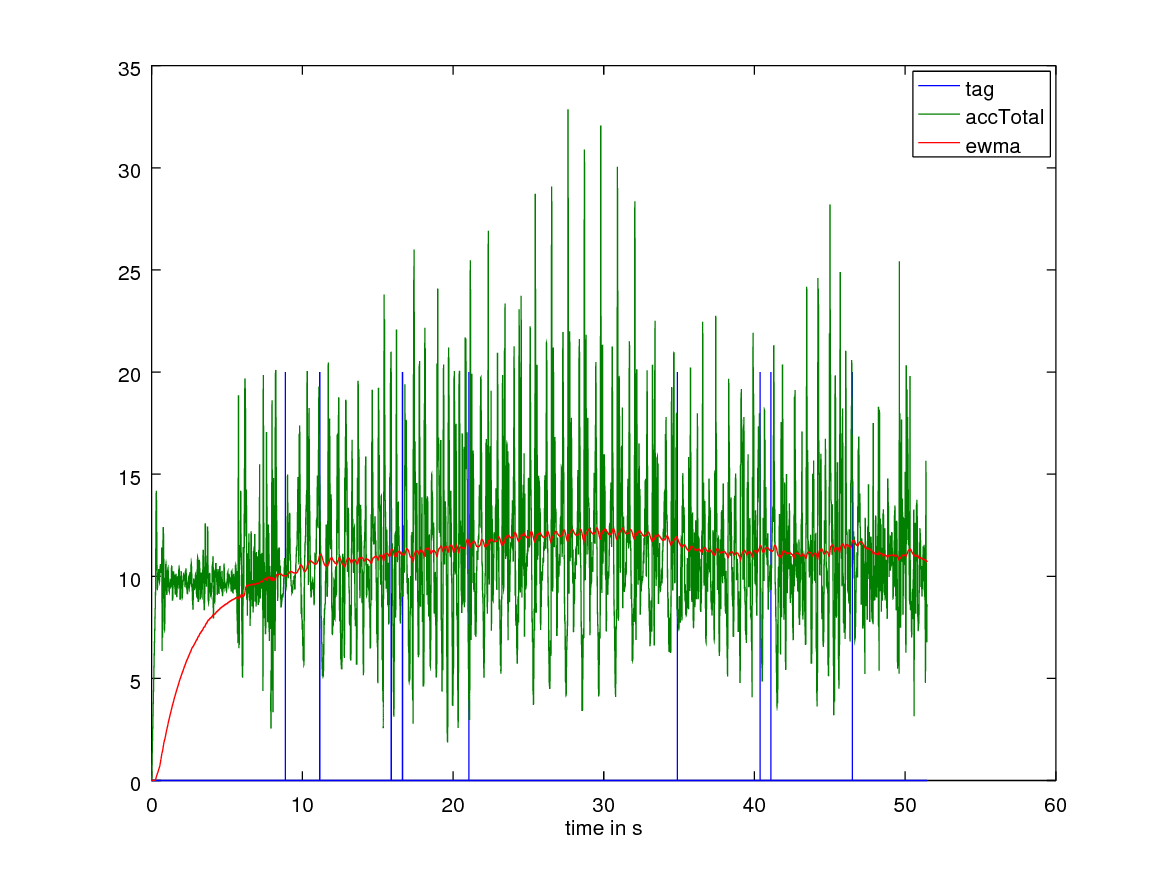
\includegraphics[width=.45\textwidth]{stairsfhdown10_atotal} &
		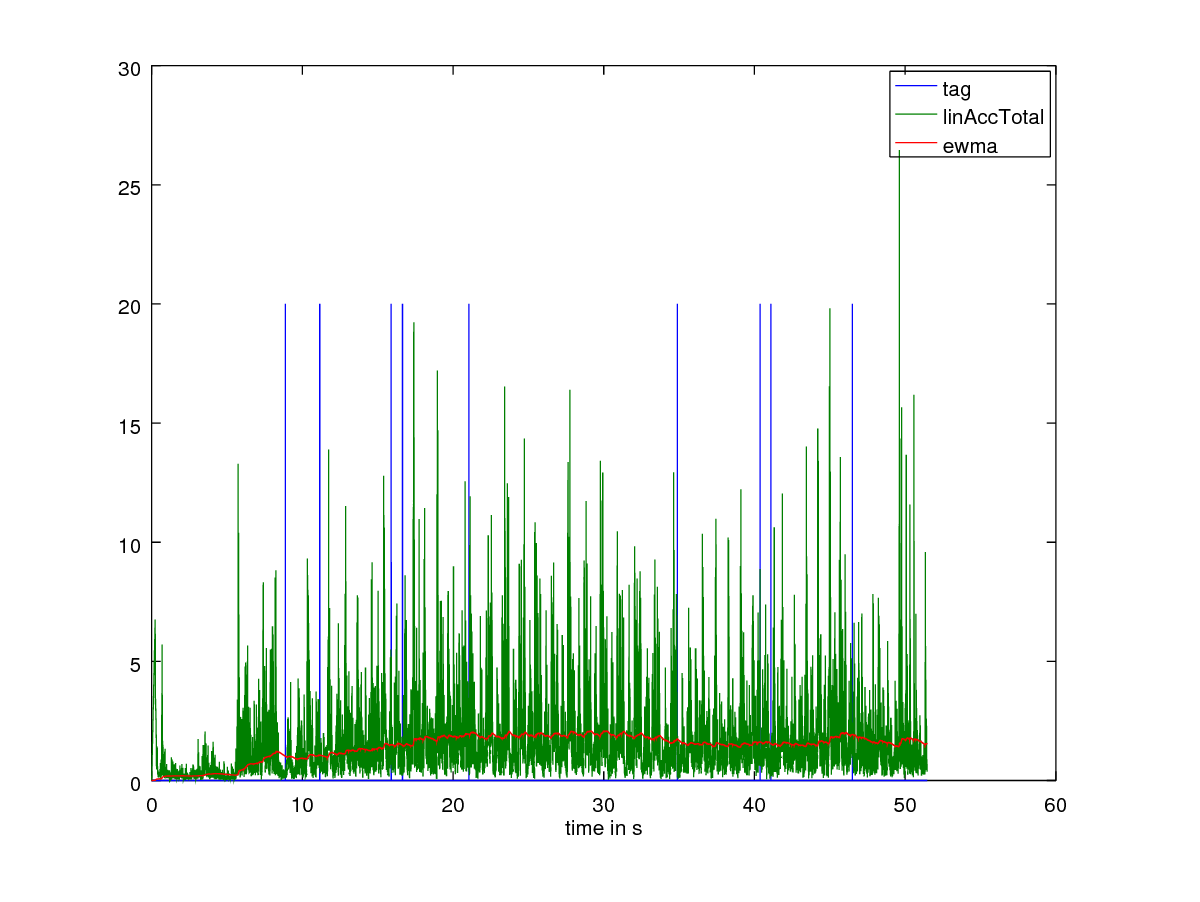
\includegraphics[width=.45\textwidth]{stairsfhdown10_latotal} 
		\\
		(e) & (f)
	\end{tabular}
	%
	\caption{Test case 4}
	\label{fig:Test_case_stairs_4}
\end{figure}

%%%----------------------------------------------------------
\section{Test case 5}
%%%----------------------------------------------------------
Test case 5 in Fig.~\ref{fig:Test_case_stairs_5}
\begin{figure}
	\centering\small
	\setlength{\tabcolsep}{0mm}	% alle Spaltenränder auf 0mm
	\begin{tabular}{c@{\hspace{12mm}}c} % mittlerer Abstand = 12mm
		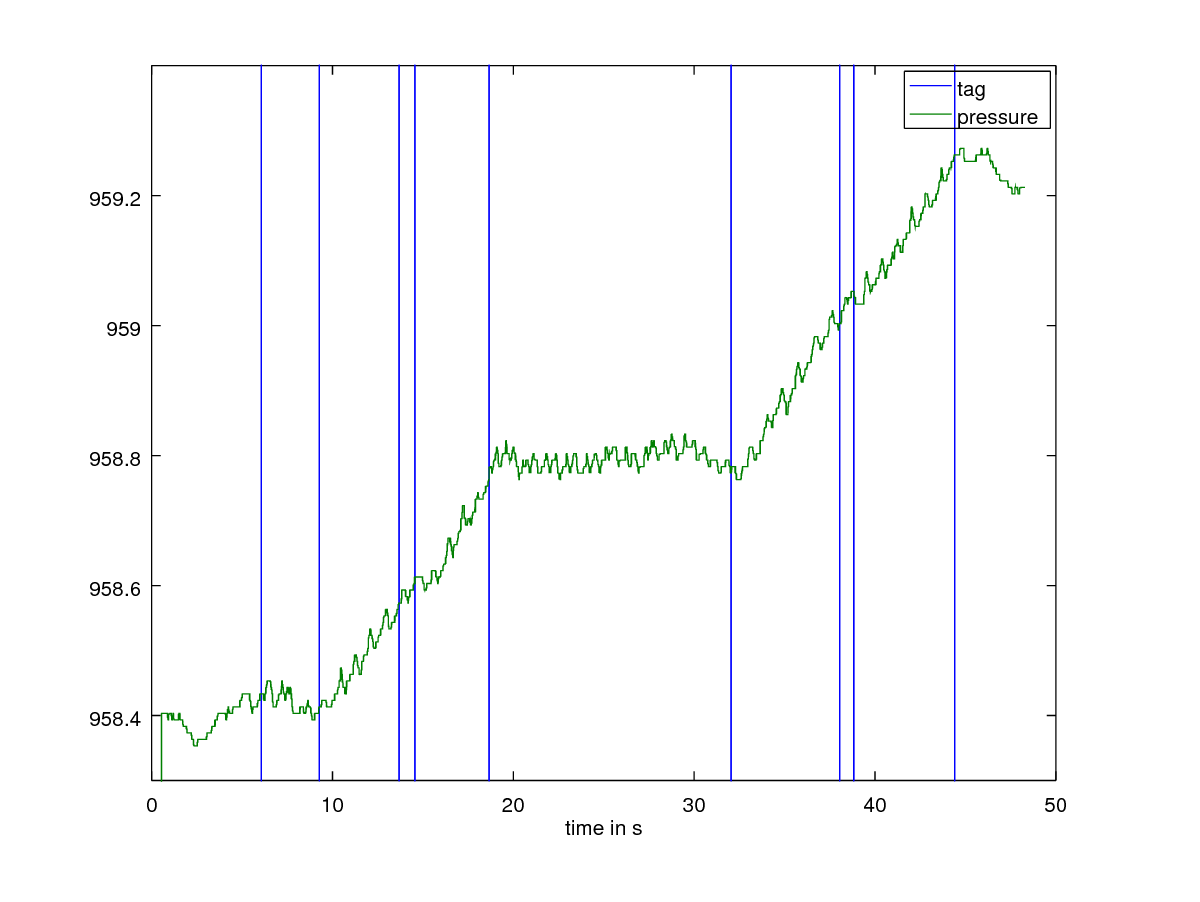
\includegraphics[width=.45\textwidth]{stairsfhdown20_p} &
		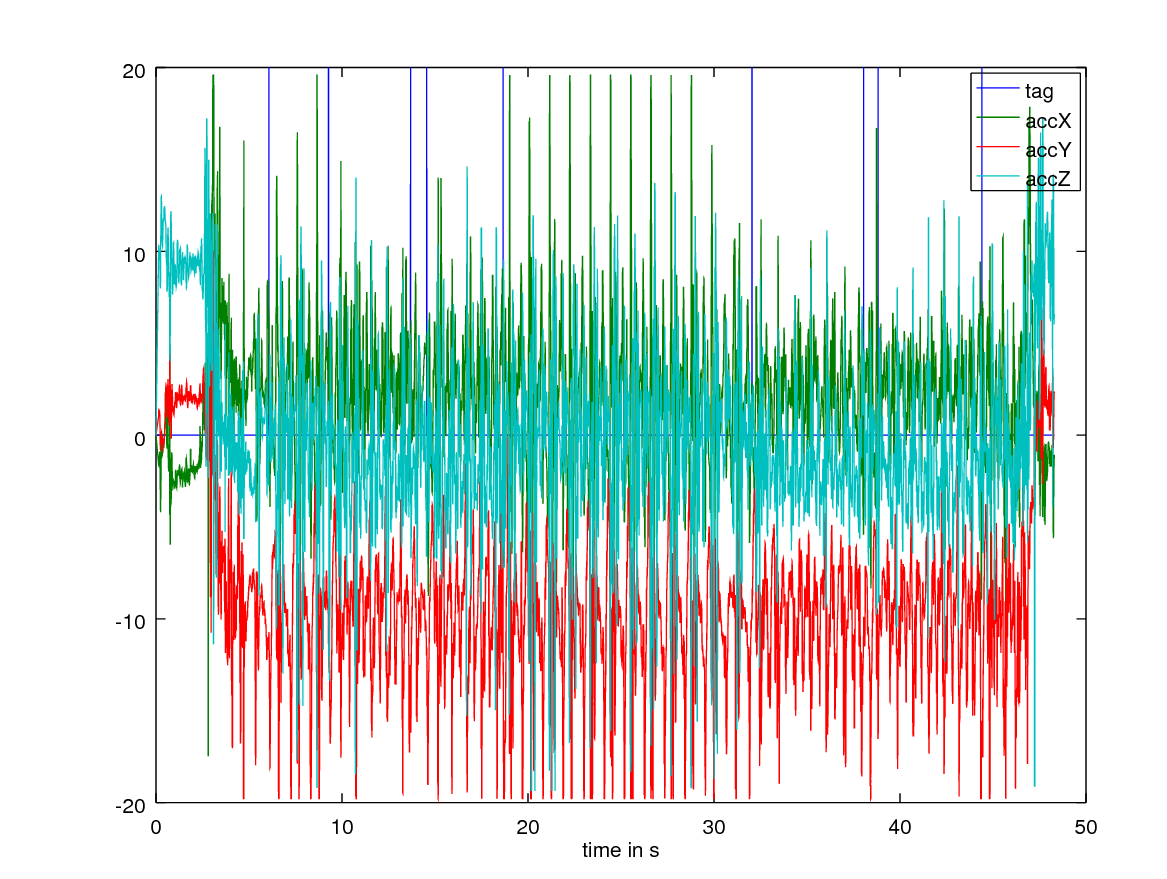
\includegraphics[width=.45\textwidth]{stairsfhdown20_a} 
		\\
		(a) & (b)
		\\[4pt]	%vertical extra spacing (4 points)
		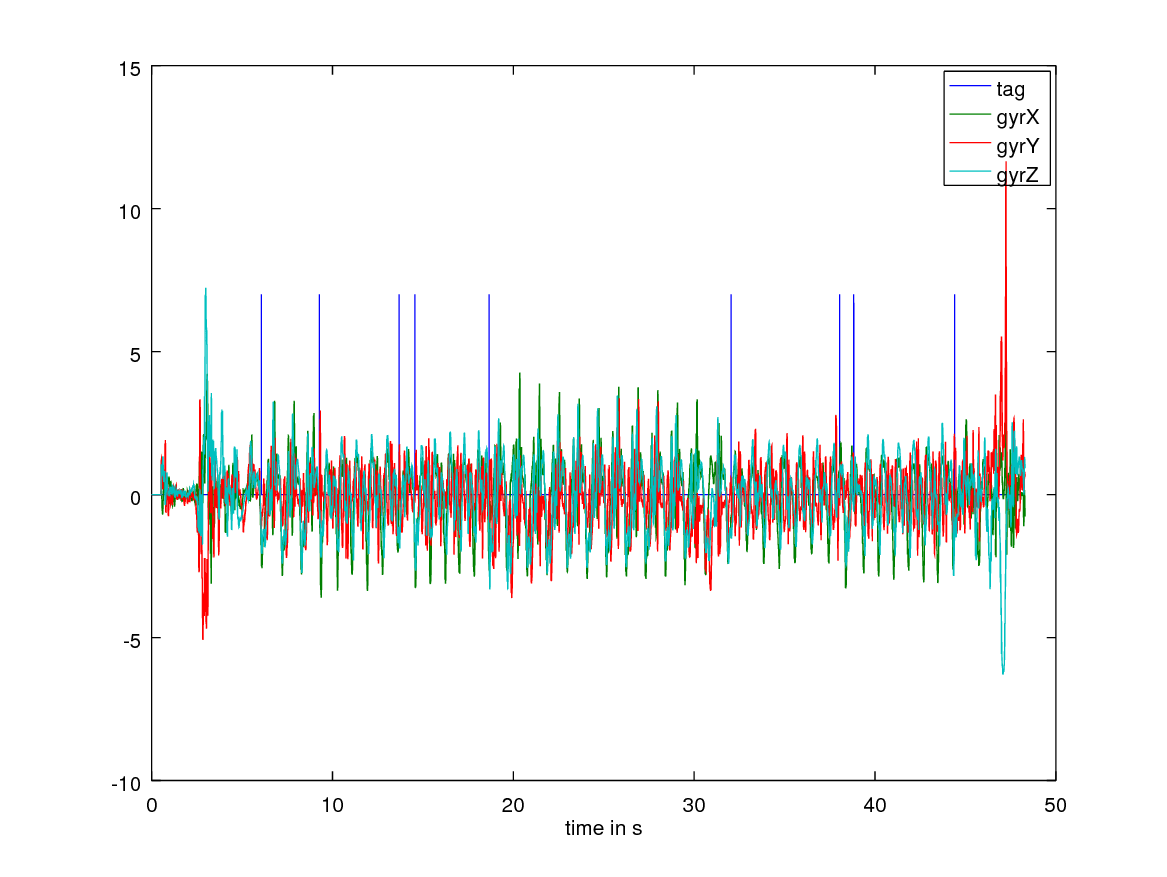
\includegraphics[width=.45\textwidth]{stairsfhdown20_g} &
		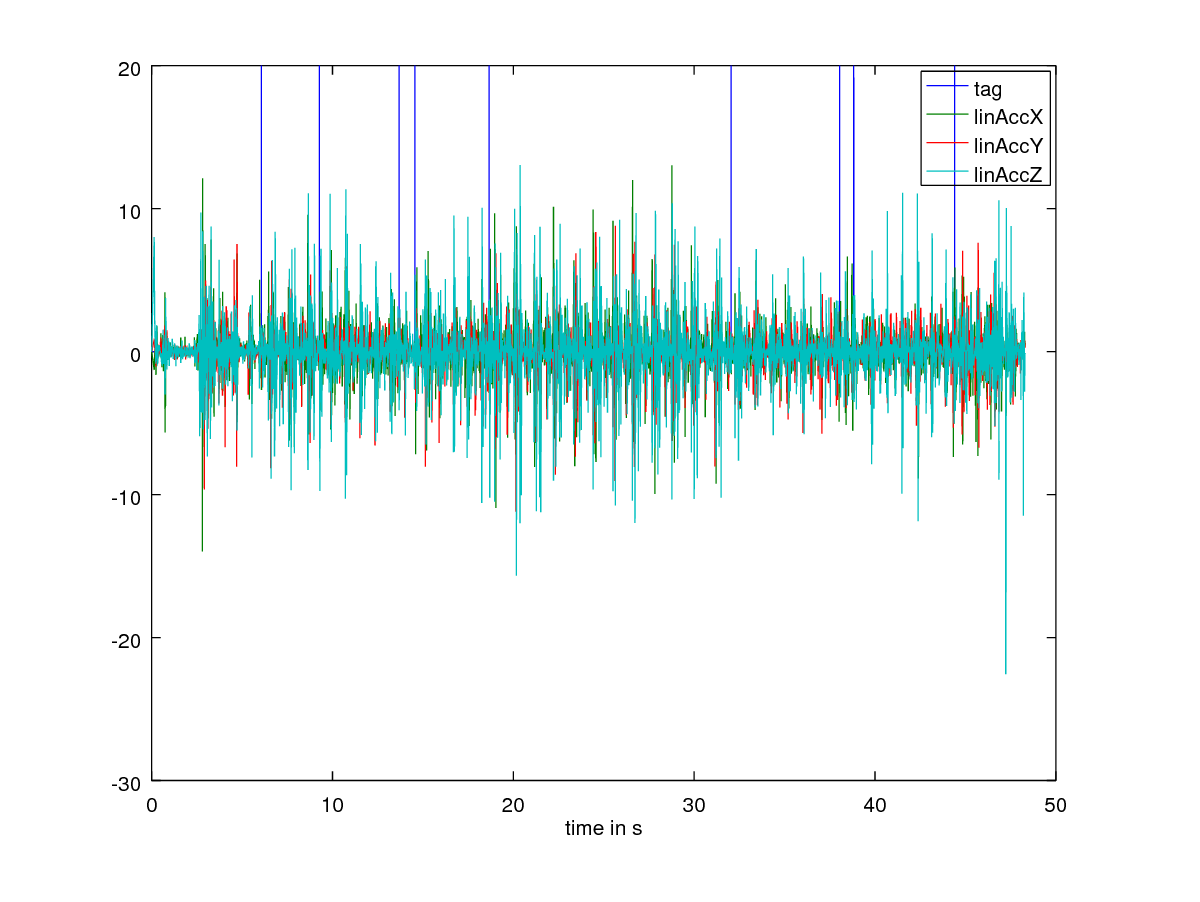
\includegraphics[width=.45\textwidth]{stairsfhdown20_la} 
		\\
		(c) & (d)
		\\[4pt]	%vertical extra spacing (4 points)
		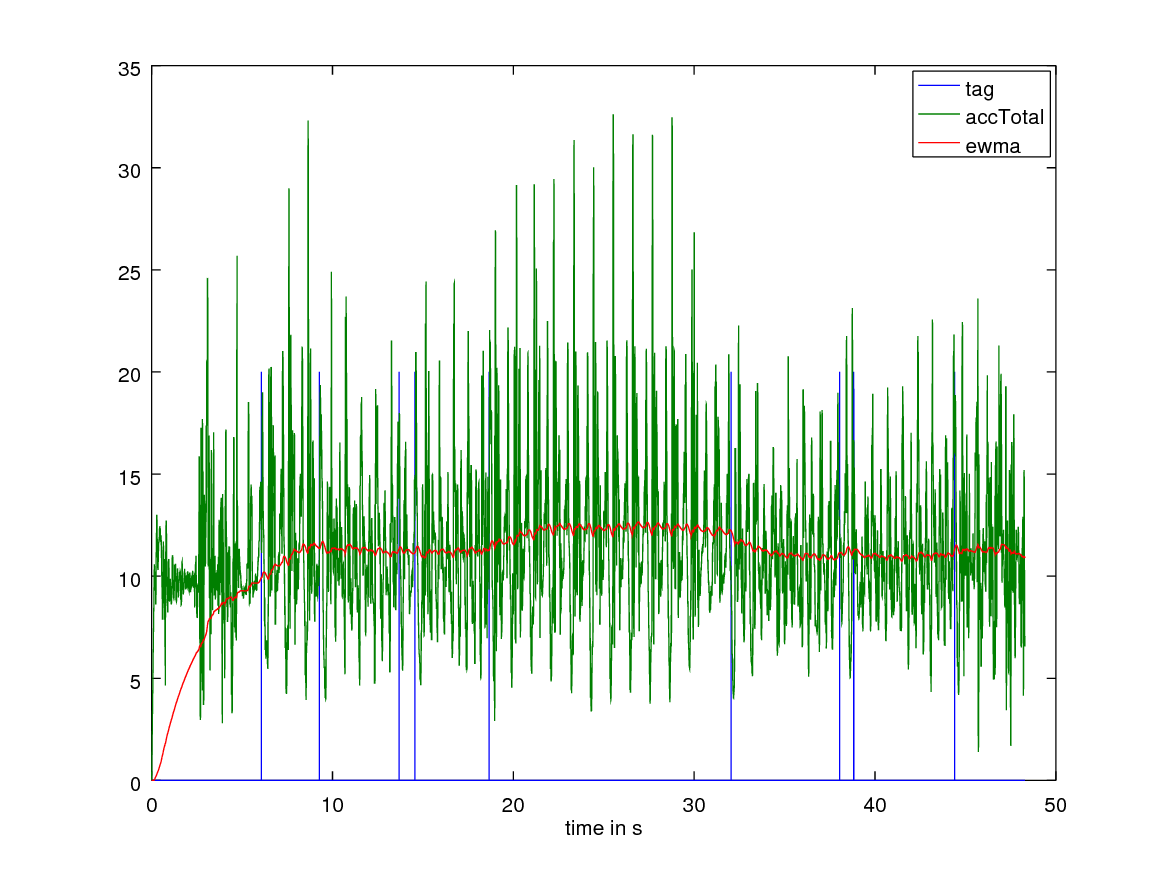
\includegraphics[width=.45\textwidth]{stairsfhdown20_atotal} &
		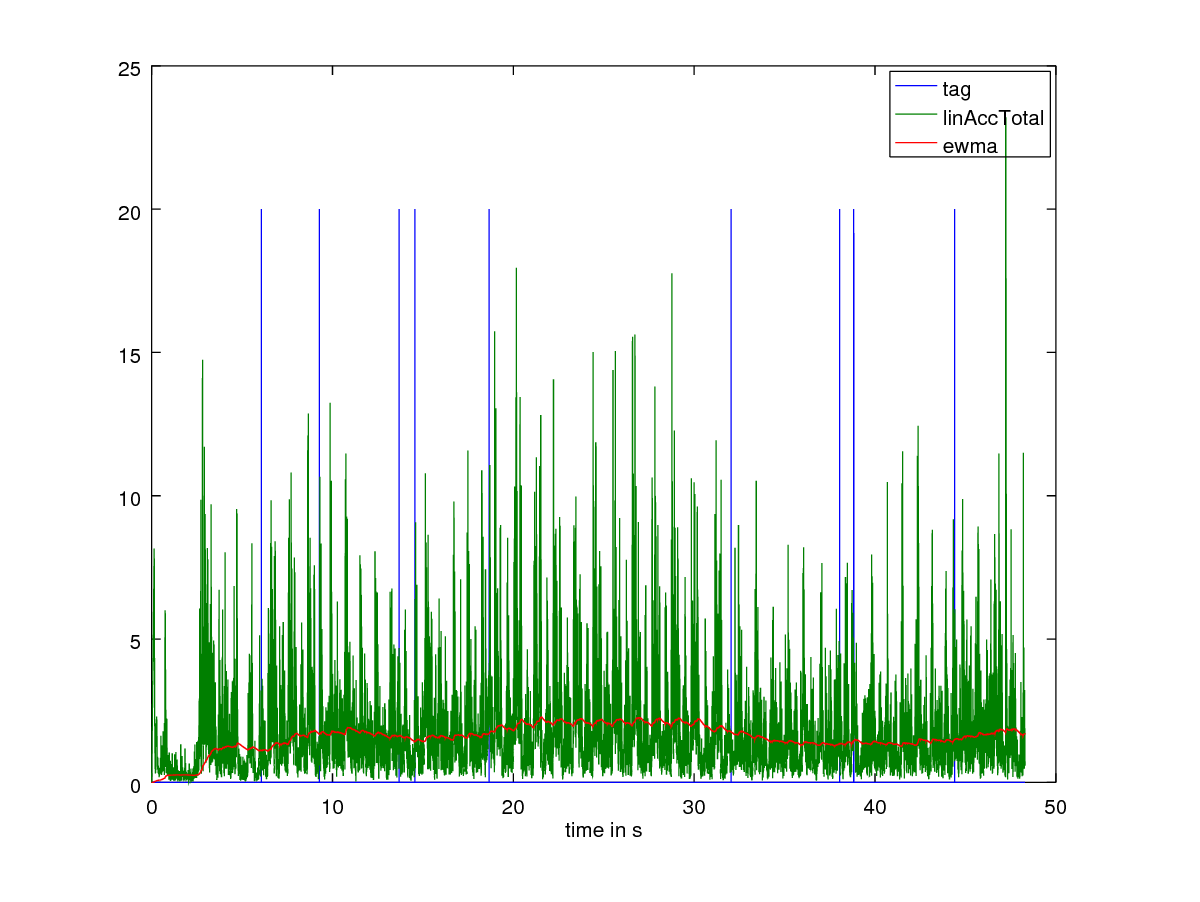
\includegraphics[width=.45\textwidth]{stairsfhdown20_latotal} 
		\\
		(e) & (f)
	\end{tabular}
	%
	\caption{Test case 5}
	\label{fig:Test_case_stairs_5}
\end{figure}

%%%----------------------------------------------------------
\section{Test case 6}
%%%----------------------------------------------------------
Test case 6 in Fig.~\ref{fig:Test_case_stairs_6}
\begin{figure}
	\centering\small
	\setlength{\tabcolsep}{0mm}	% alle Spaltenränder auf 0mm
	\begin{tabular}{c@{\hspace{12mm}}c} % mittlerer Abstand = 12mm
		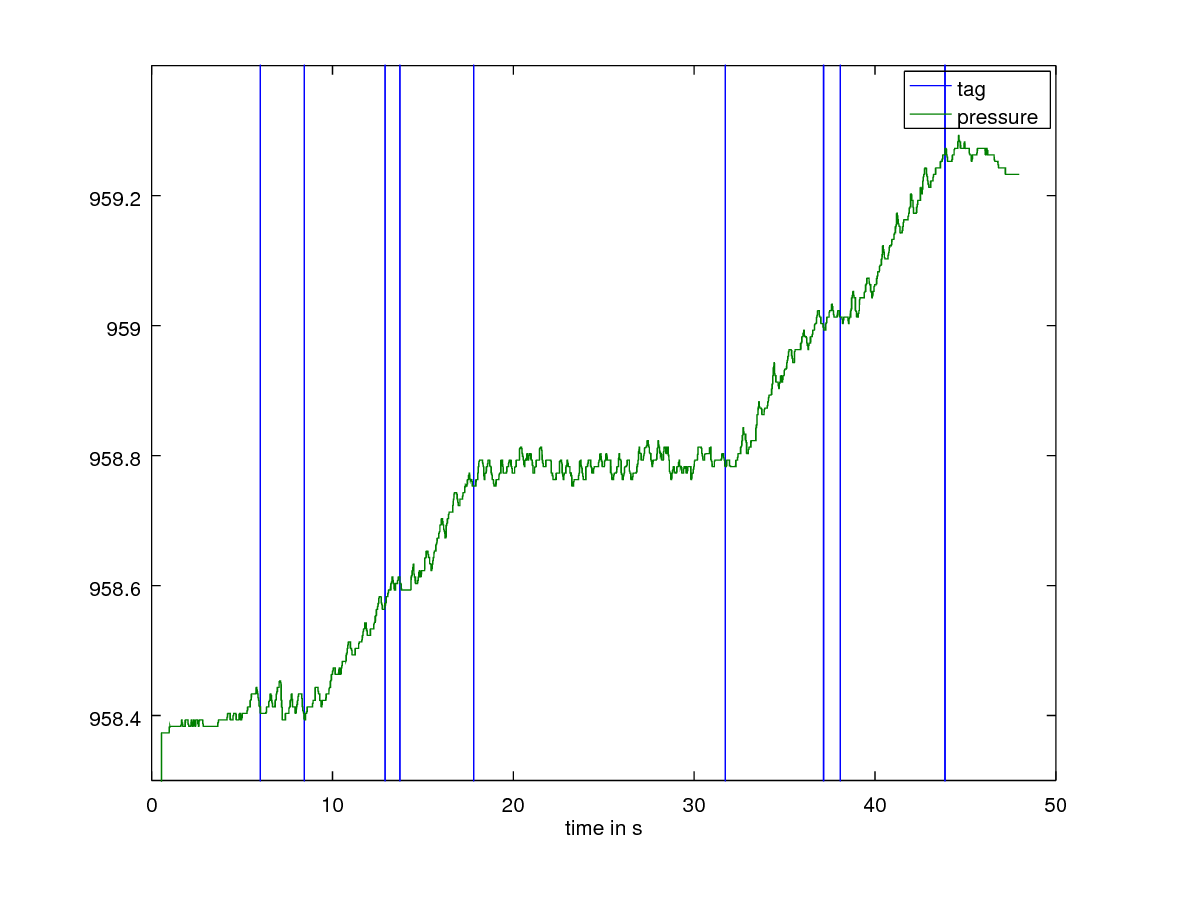
\includegraphics[width=.45\textwidth]{stairsfhdown50_p} &
		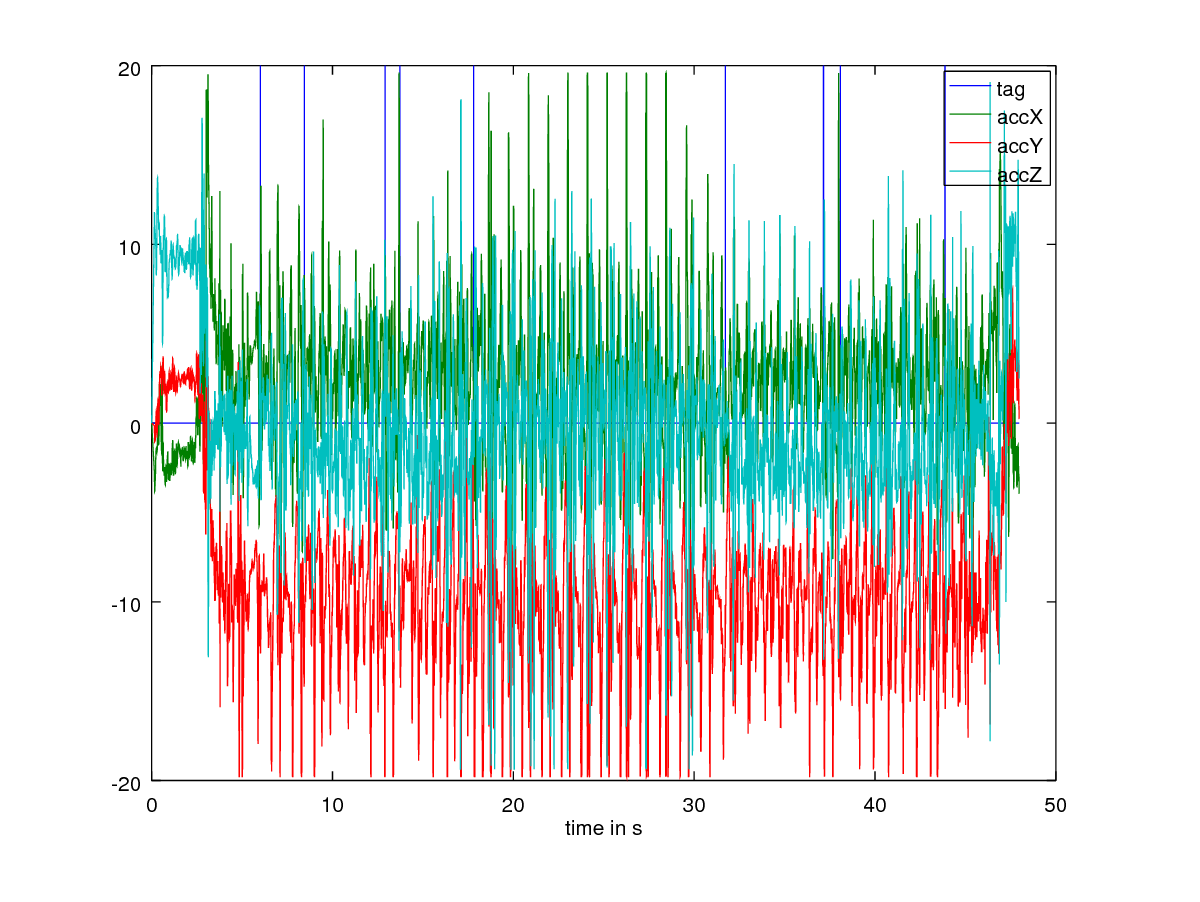
\includegraphics[width=.45\textwidth]{stairsfhdown50_a} 
		\\
		(a) & (b)
		\\[4pt]	%vertical extra spacing (4 points)
		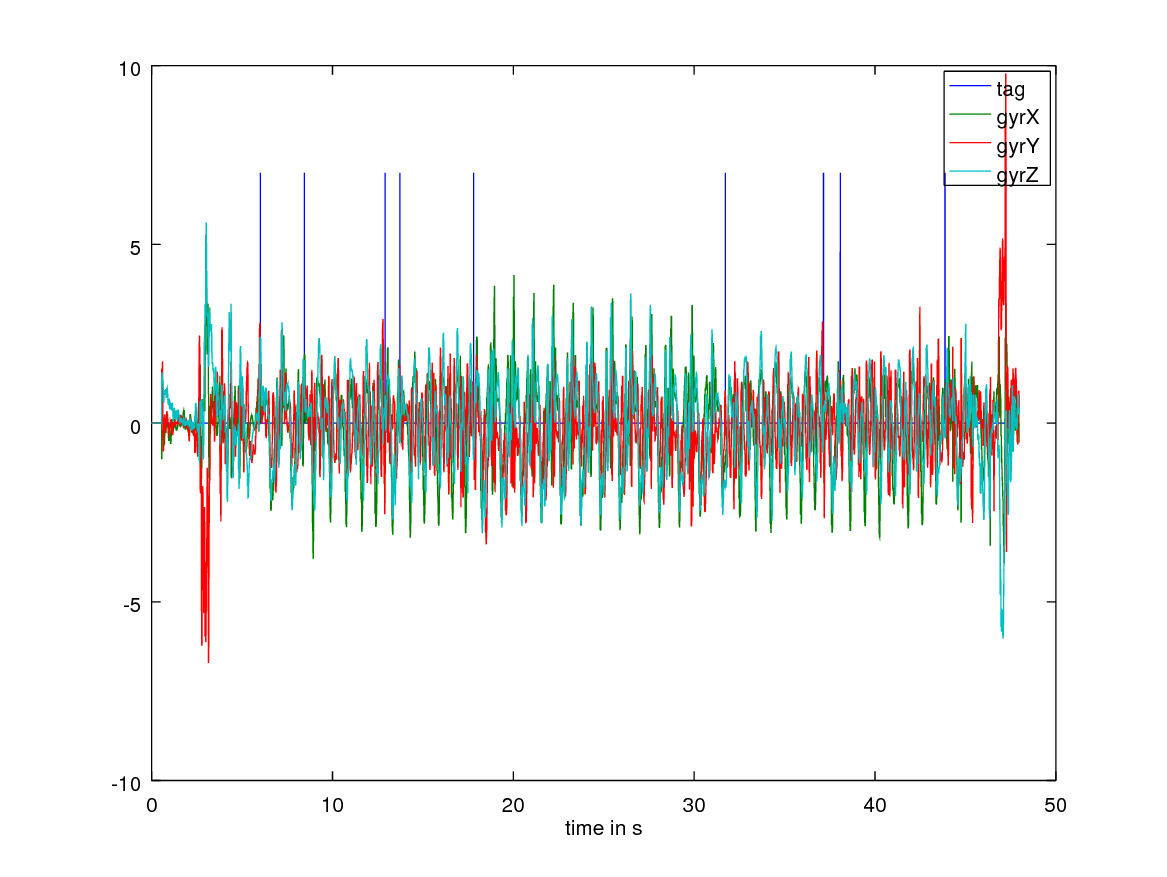
\includegraphics[width=.45\textwidth]{stairsfhdown50_g} &
		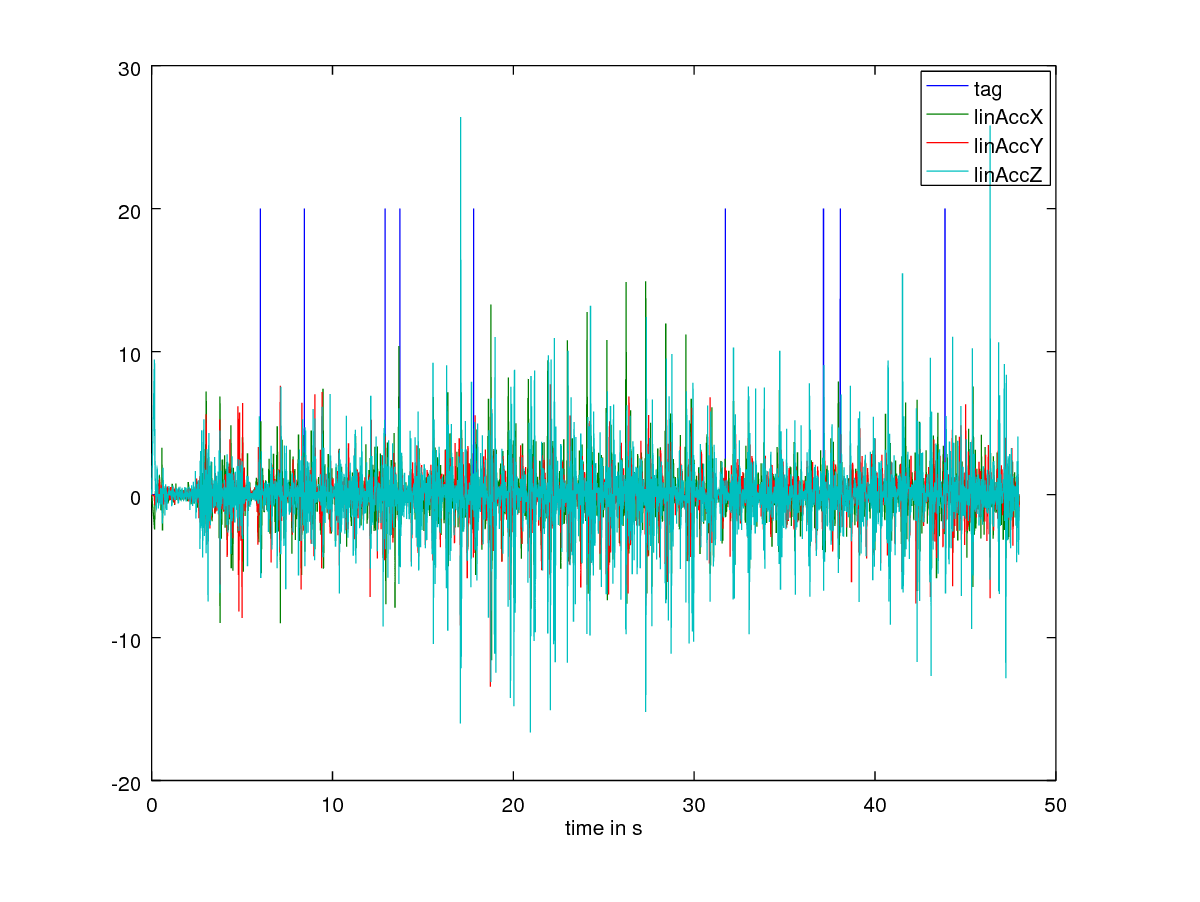
\includegraphics[width=.45\textwidth]{stairsfhdown50_la} 
		\\
		(c) & (d)
		\\[4pt]	%vertical extra spacing (4 points)
		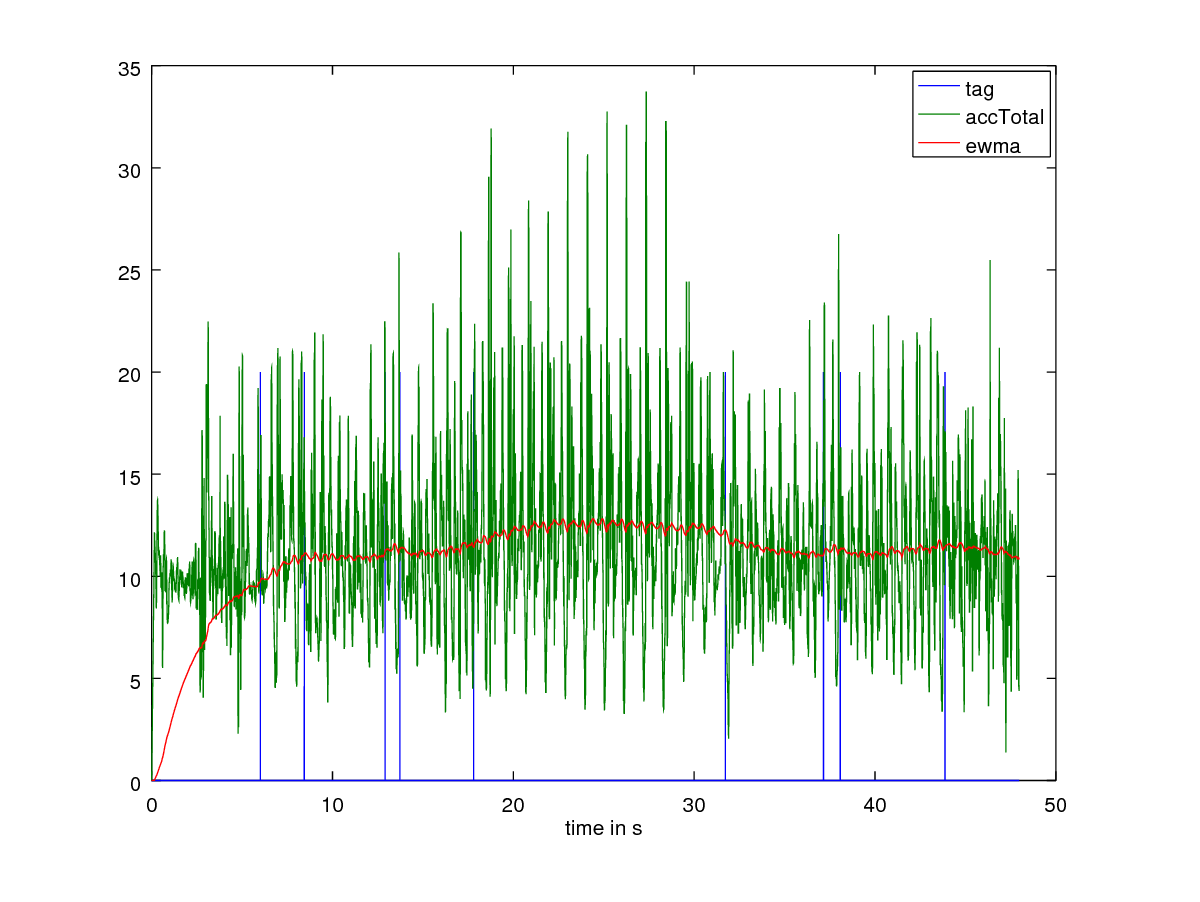
\includegraphics[width=.45\textwidth]{stairsfhdown50_atotal} &
		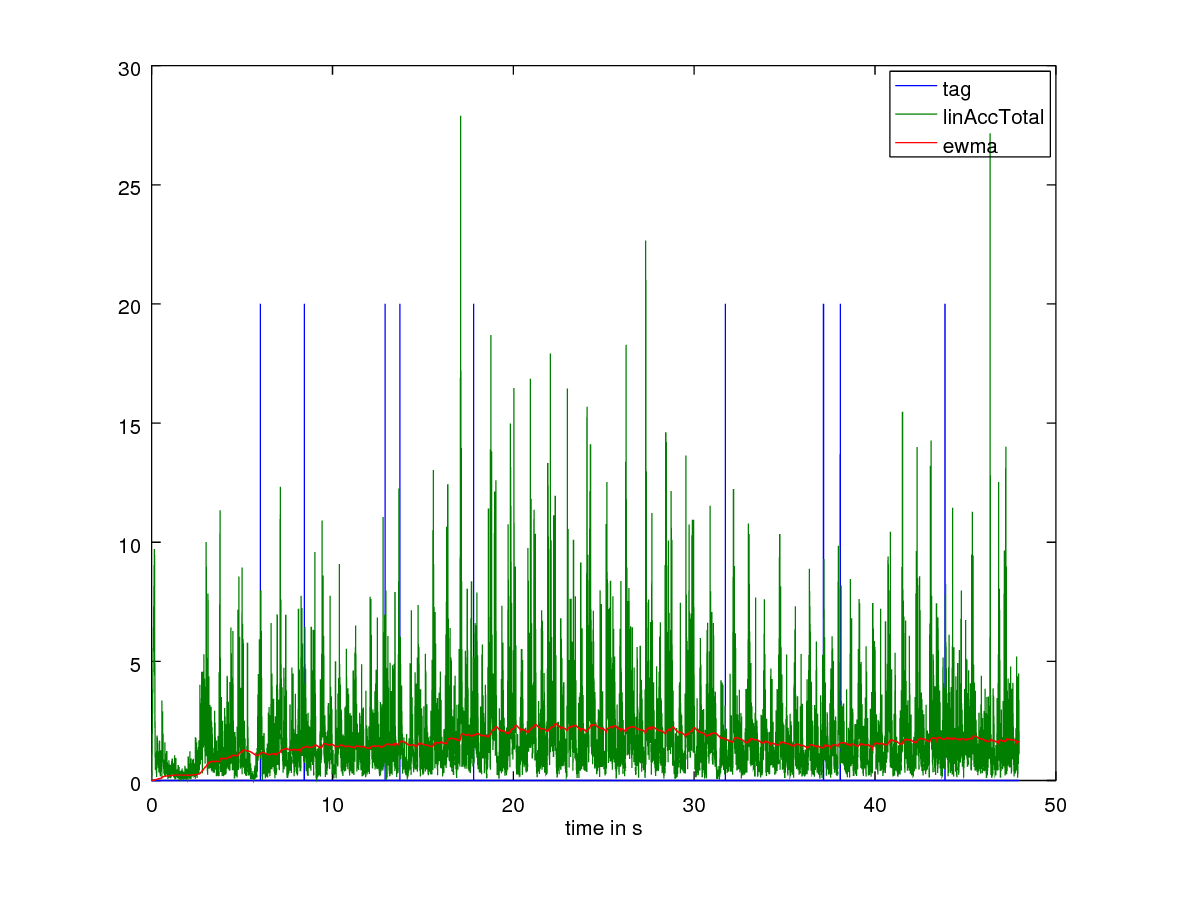
\includegraphics[width=.45\textwidth]{stairsfhdown50_latotal} 
		\\
		(e) & (f)
	\end{tabular}
	%
	\caption{Test case 6}
	\label{fig:Test_case_stairs_6}
\end{figure}


%%%----------------------------------------------------------
\section{Test case 7}
%%%----------------------------------------------------------
Test case 7 in Fig.~\ref{fig:Test_case_stairs_7}
\begin{figure}
	\centering\small
	\setlength{\tabcolsep}{0mm}	% alle Spaltenränder auf 0mm
	\begin{tabular}{c@{\hspace{12mm}}c} % mittlerer Abstand = 12mm
		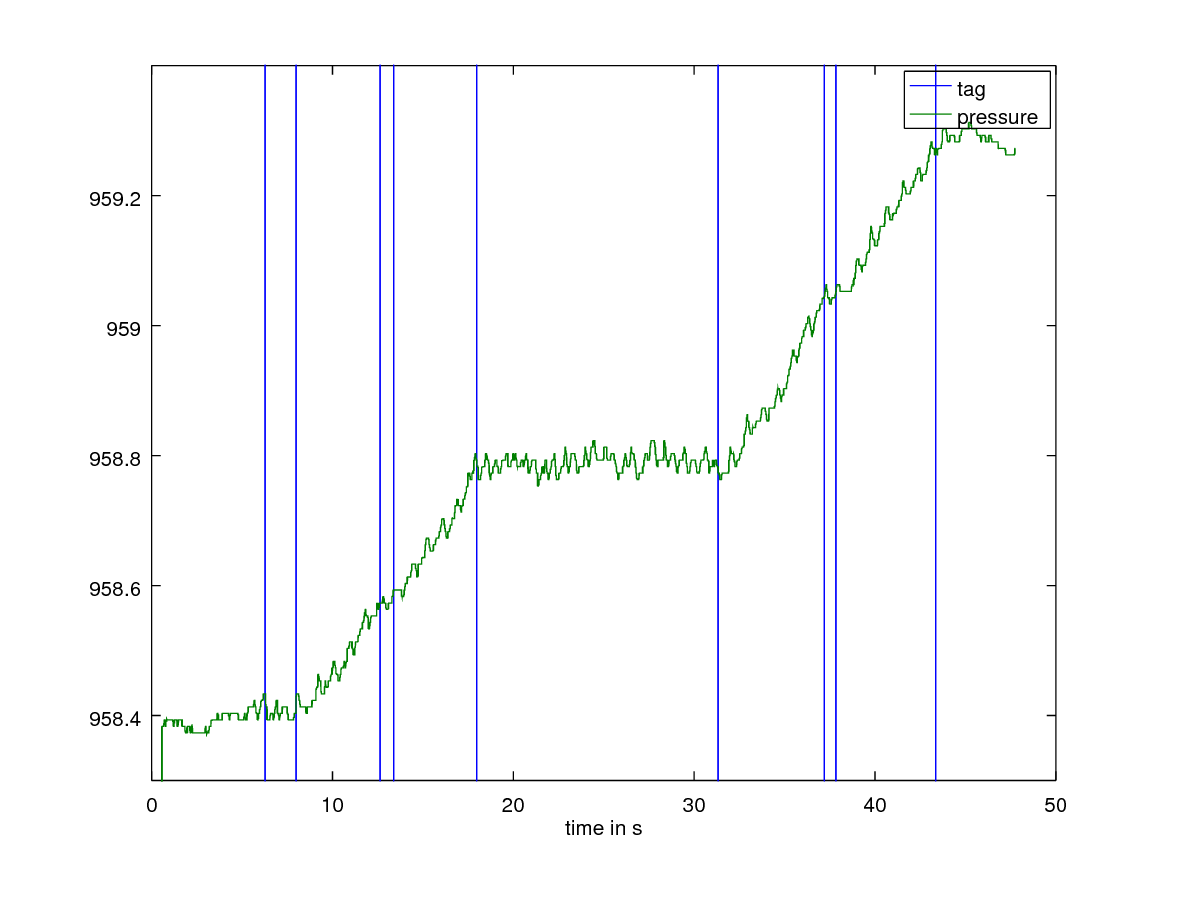
\includegraphics[width=.45\textwidth]{stairsfhdown70_p} &
		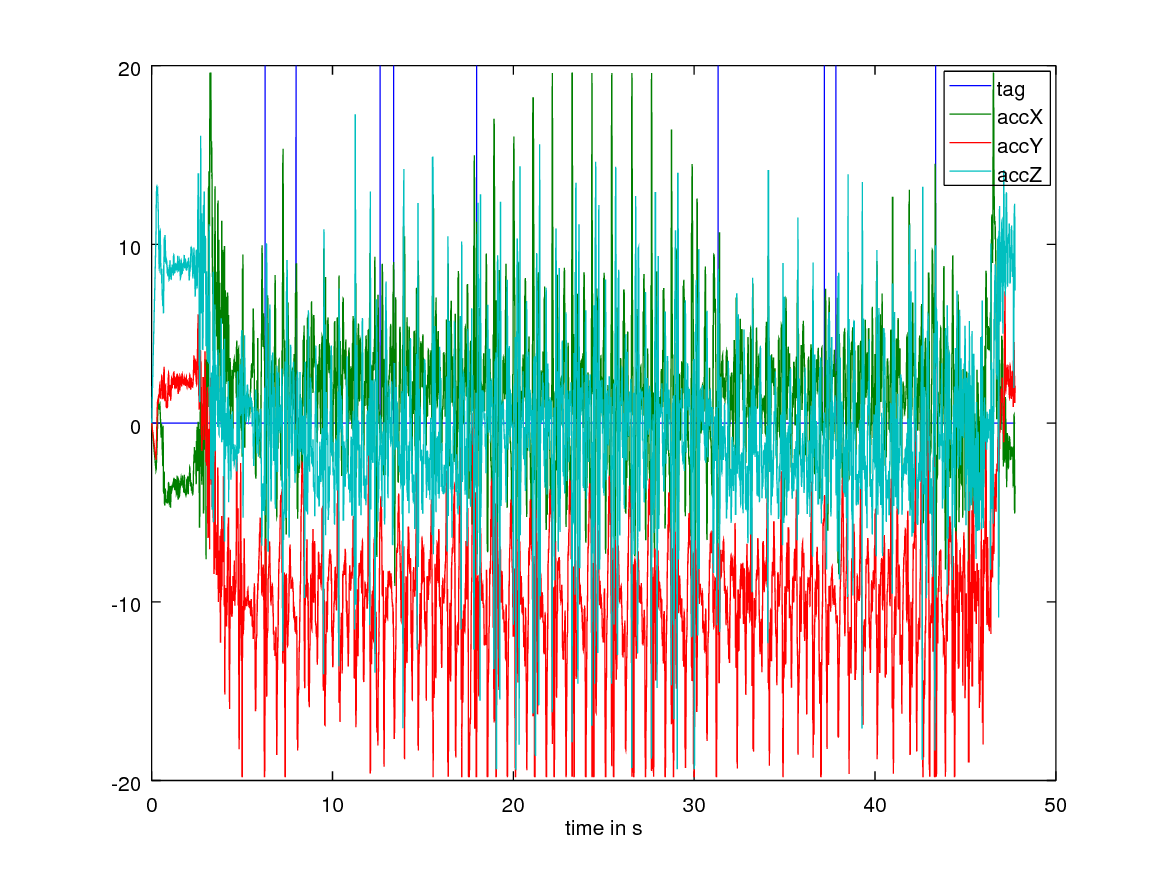
\includegraphics[width=.45\textwidth]{stairsfhdown70_a} 
		\\
		(a) & (b)
		\\[4pt]	%vertical extra spacing (4 points)
		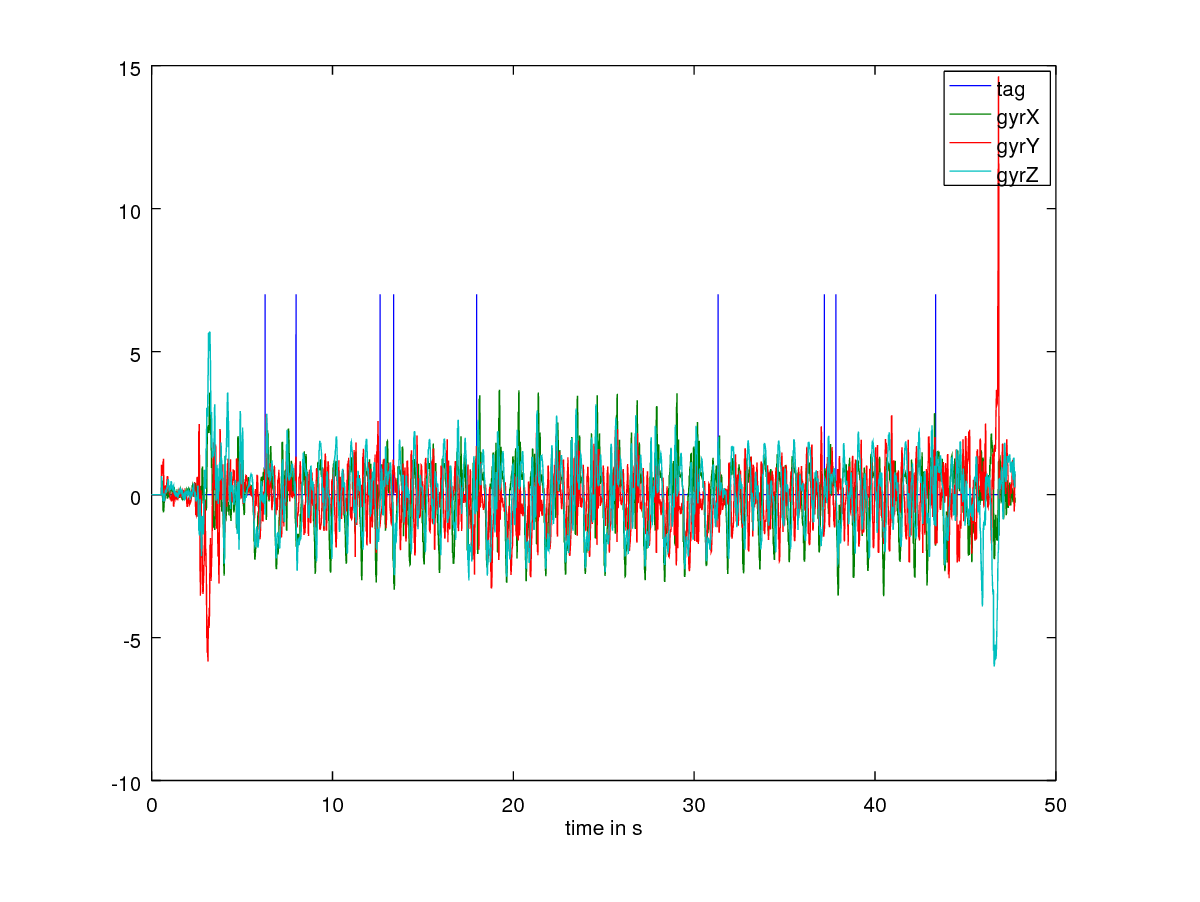
\includegraphics[width=.45\textwidth]{stairsfhdown70_g} &
		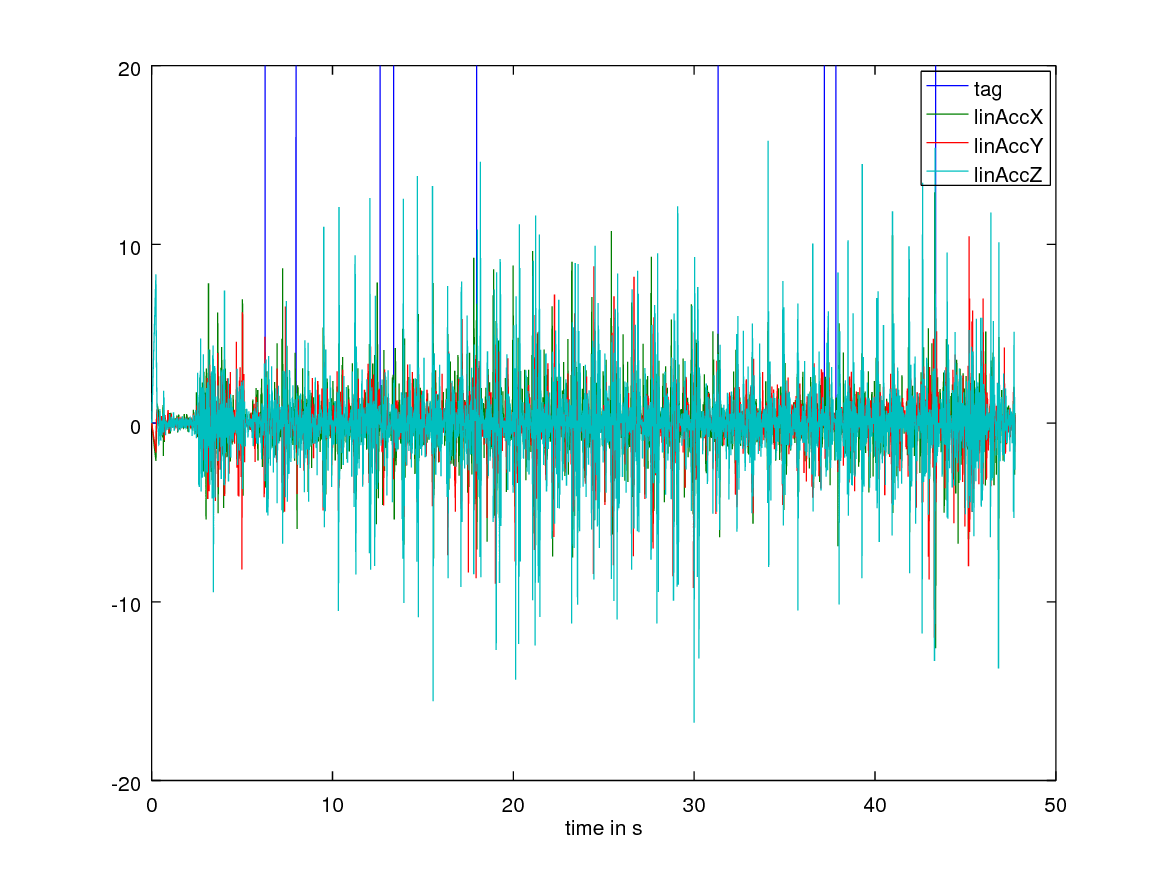
\includegraphics[width=.45\textwidth]{stairsfhdown70_la} 
		\\
		(c) & (d)
		\\[4pt]	%vertical extra spacing (4 points)
		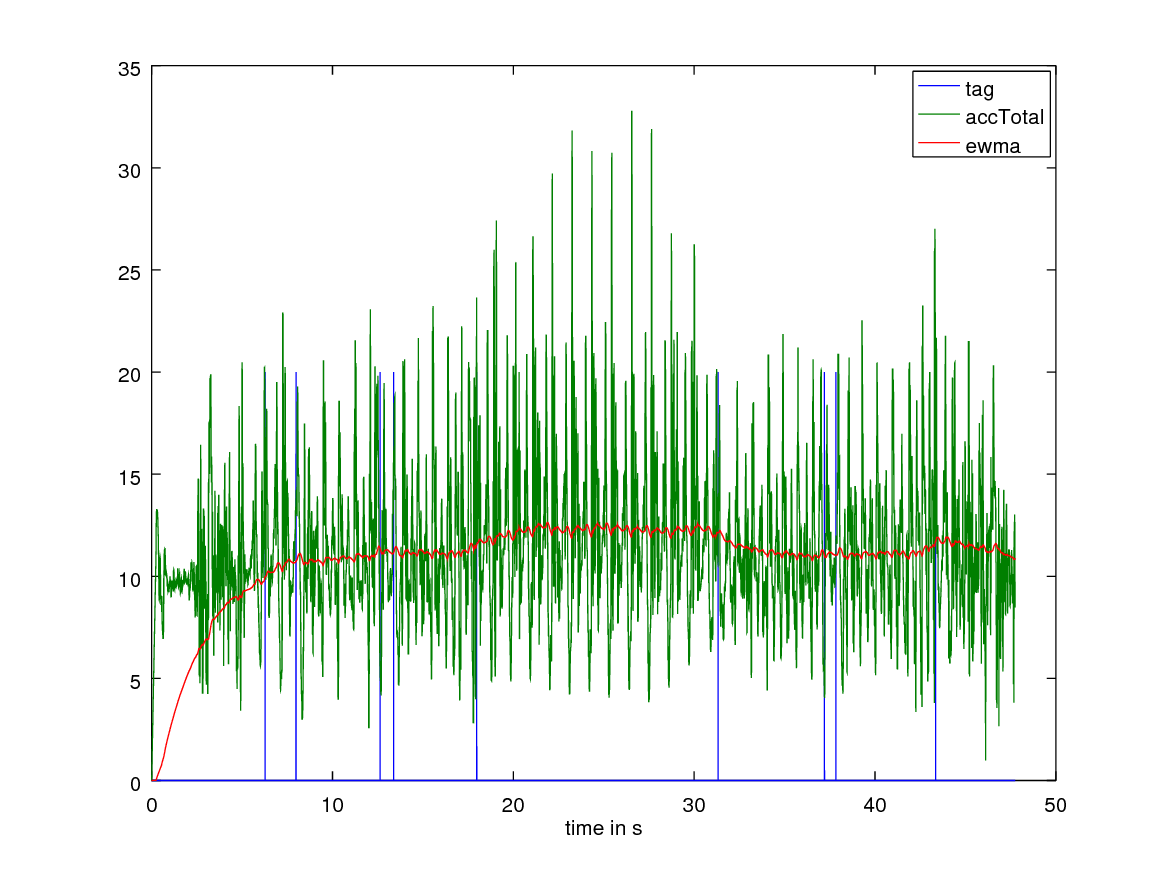
\includegraphics[width=.45\textwidth]{stairsfhdown70_atotal} &
		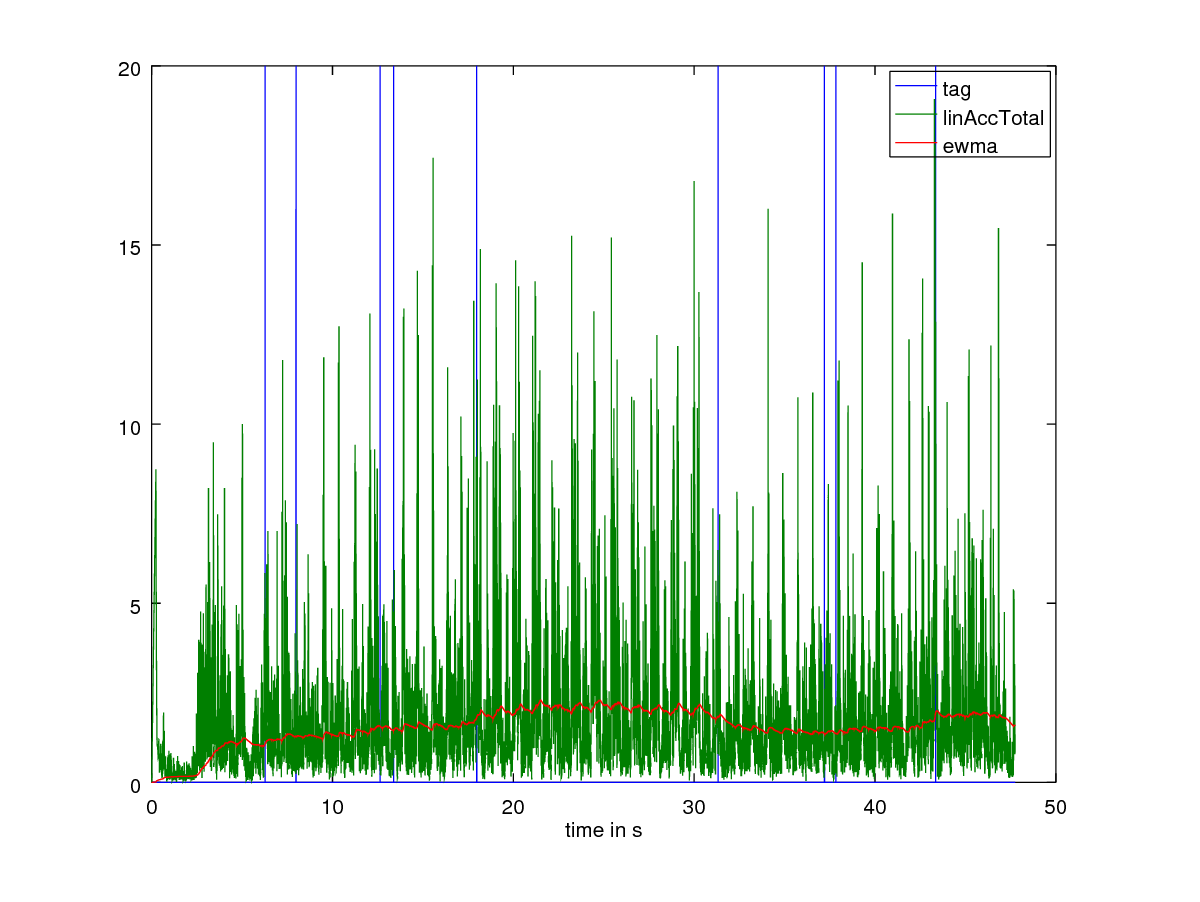
\includegraphics[width=.45\textwidth]{stairsfhdown70_latotal} 
		\\
		(e) & (f)
	\end{tabular}
	%
	\caption{Test case 7}
	\label{fig:Test_case_stairs_7}
\end{figure}


%%%----------------------------------------------------------
\section{Test case 8}
%%%----------------------------------------------------------
Test case 8 in Fig.~\ref{fig:Test_case_stairs_8}
\begin{figure}
	\centering\small
	\setlength{\tabcolsep}{0mm}	% alle Spaltenränder auf 0mm
	\begin{tabular}{c@{\hspace{12mm}}c} % mittlerer Abstand = 12mm
		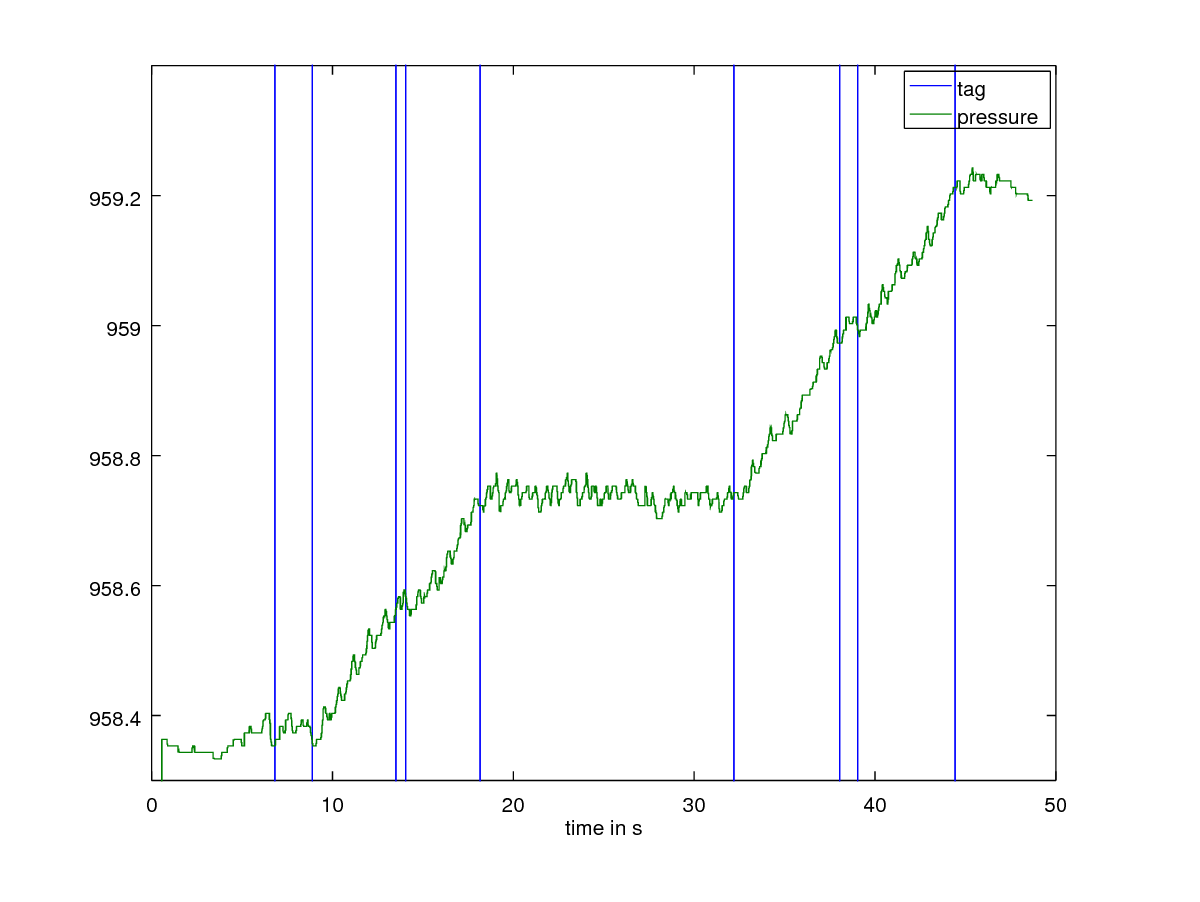
\includegraphics[width=.45\textwidth]{stairsfhdown100_p} &
		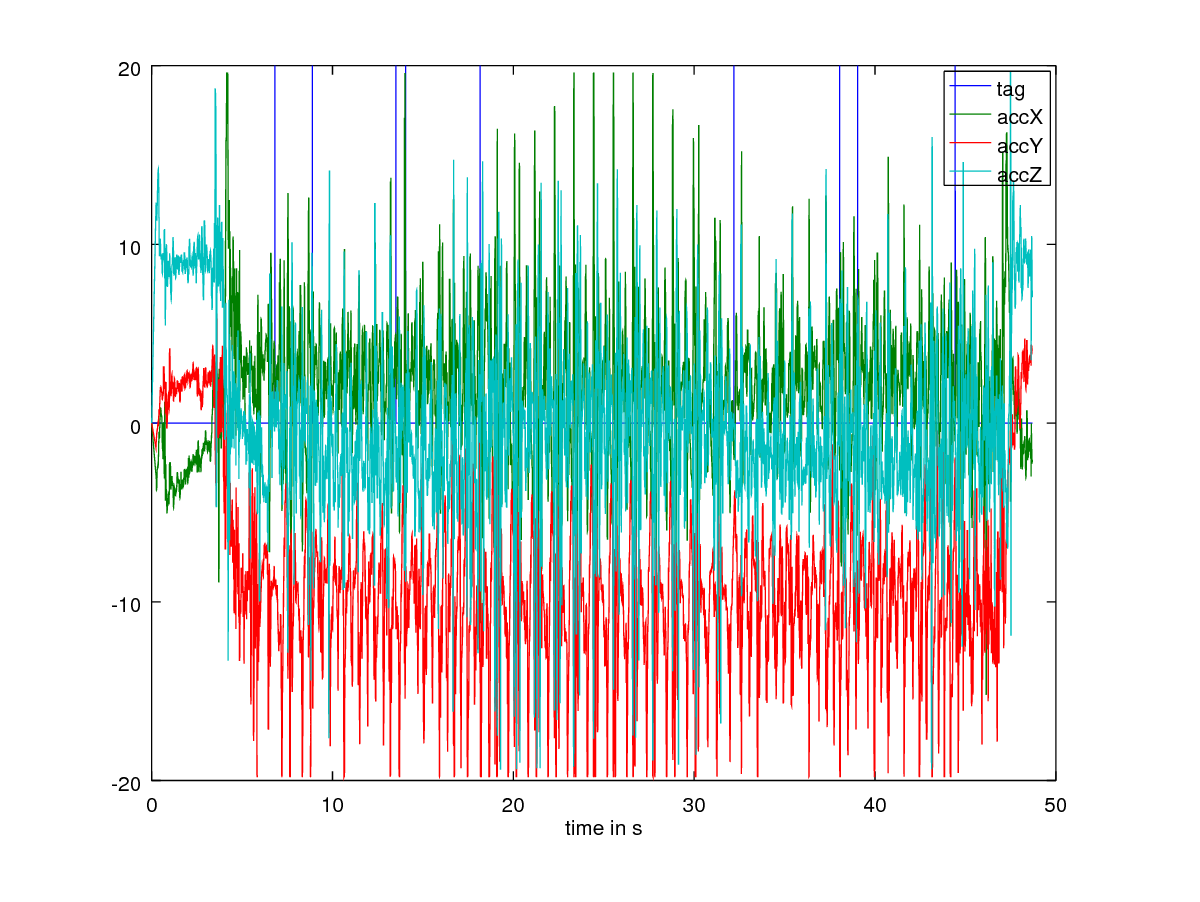
\includegraphics[width=.45\textwidth]{stairsfhdown100_a} 
		\\
		(a) & (b)
		\\[4pt]	%vertical extra spacing (4 points)
		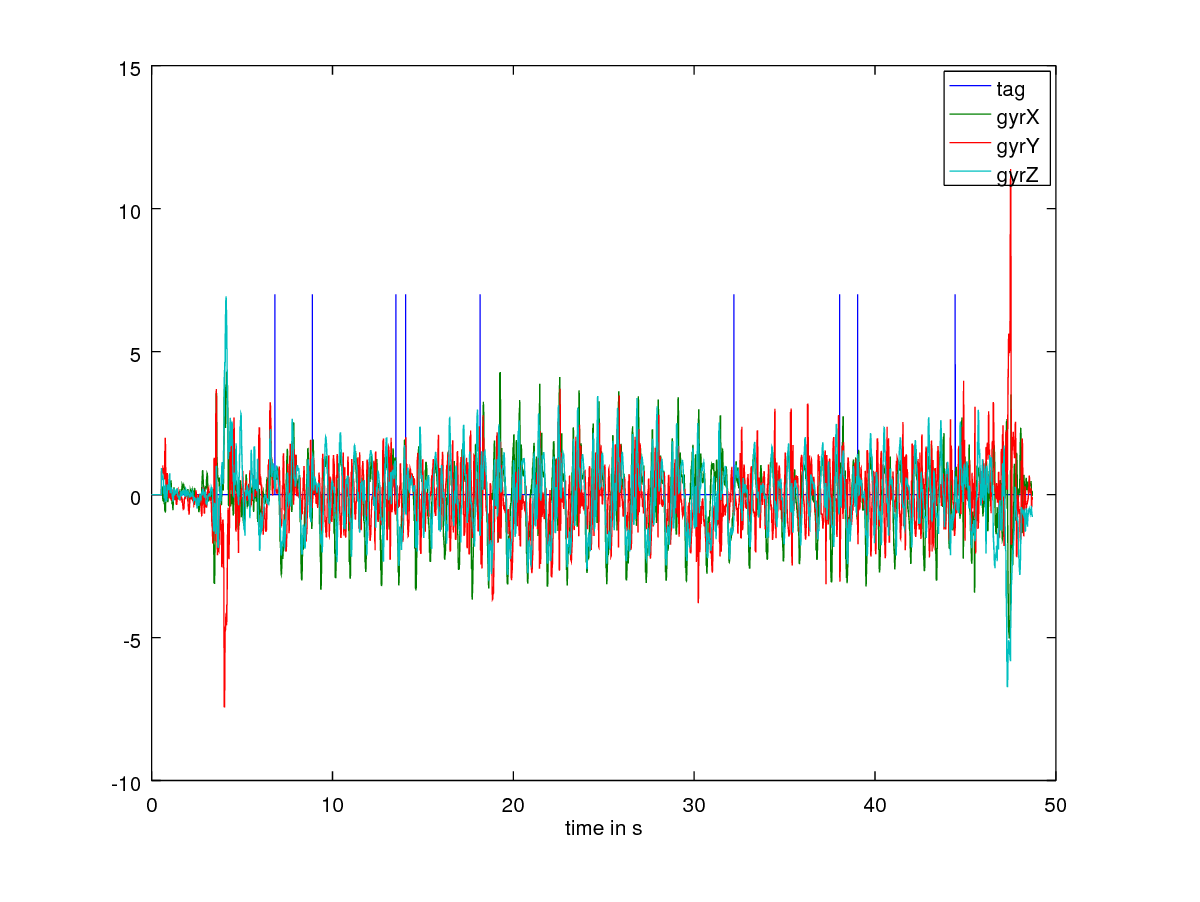
\includegraphics[width=.45\textwidth]{stairsfhdown100_g} &
		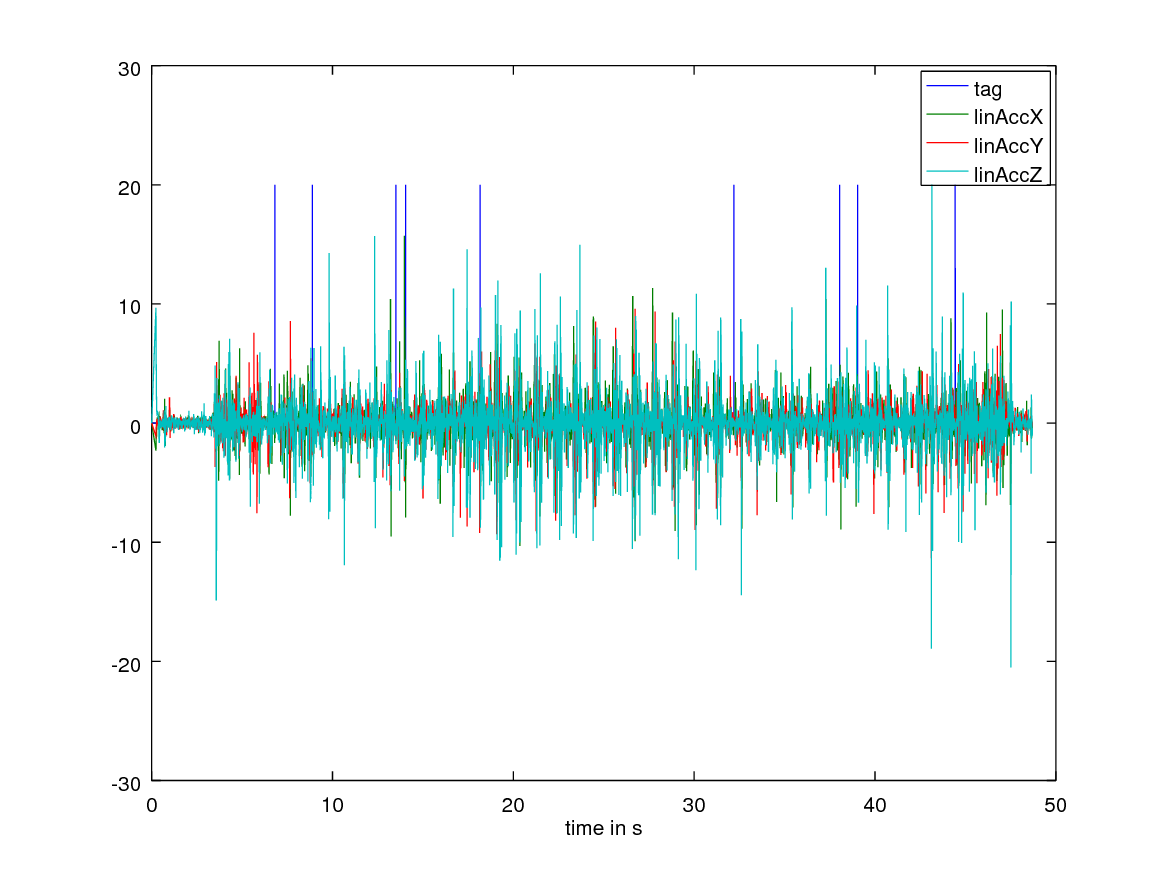
\includegraphics[width=.45\textwidth]{stairsfhdown100_la} 
		\\
		(c) & (d)
		\\[4pt]	%vertical extra spacing (4 points)
		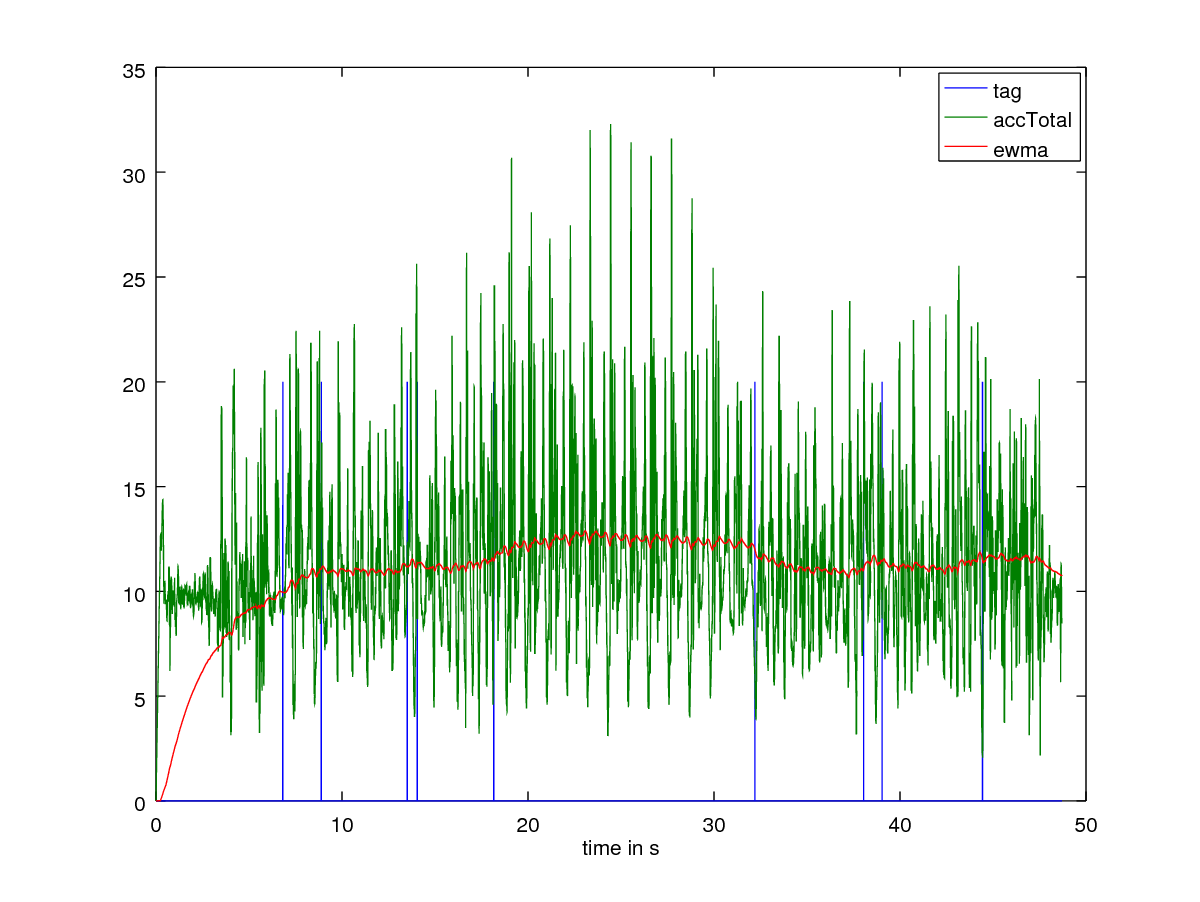
\includegraphics[width=.45\textwidth]{stairsfhdown100_atotal} &
		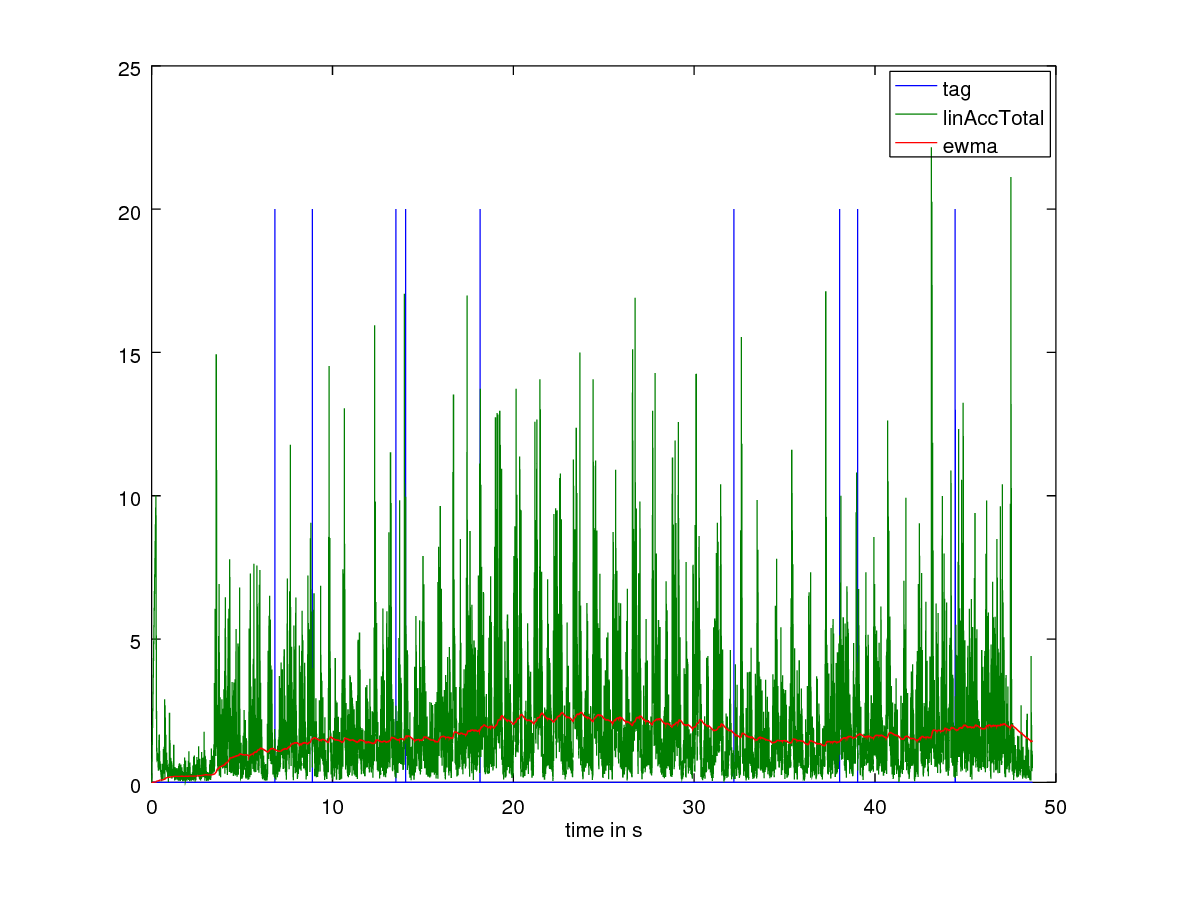
\includegraphics[width=.45\textwidth]{stairsfhdown100_latotal} 
		\\
		(e) & (f)
	\end{tabular}
	%
	\caption{Test case 8}
	\label{fig:Test_case_stairs_8}
\end{figure}

%%%----------------------------------------------------------
\section{Test case 9}
%%%----------------------------------------------------------
Test case 9 in Fig.~\ref{fig:Test_case_stairs_9}
\begin{figure}
	\centering\small
	\setlength{\tabcolsep}{0mm}	% alle Spaltenränder auf 0mm
	\begin{tabular}{c@{\hspace{12mm}}c} % mittlerer Abstand = 12mm
		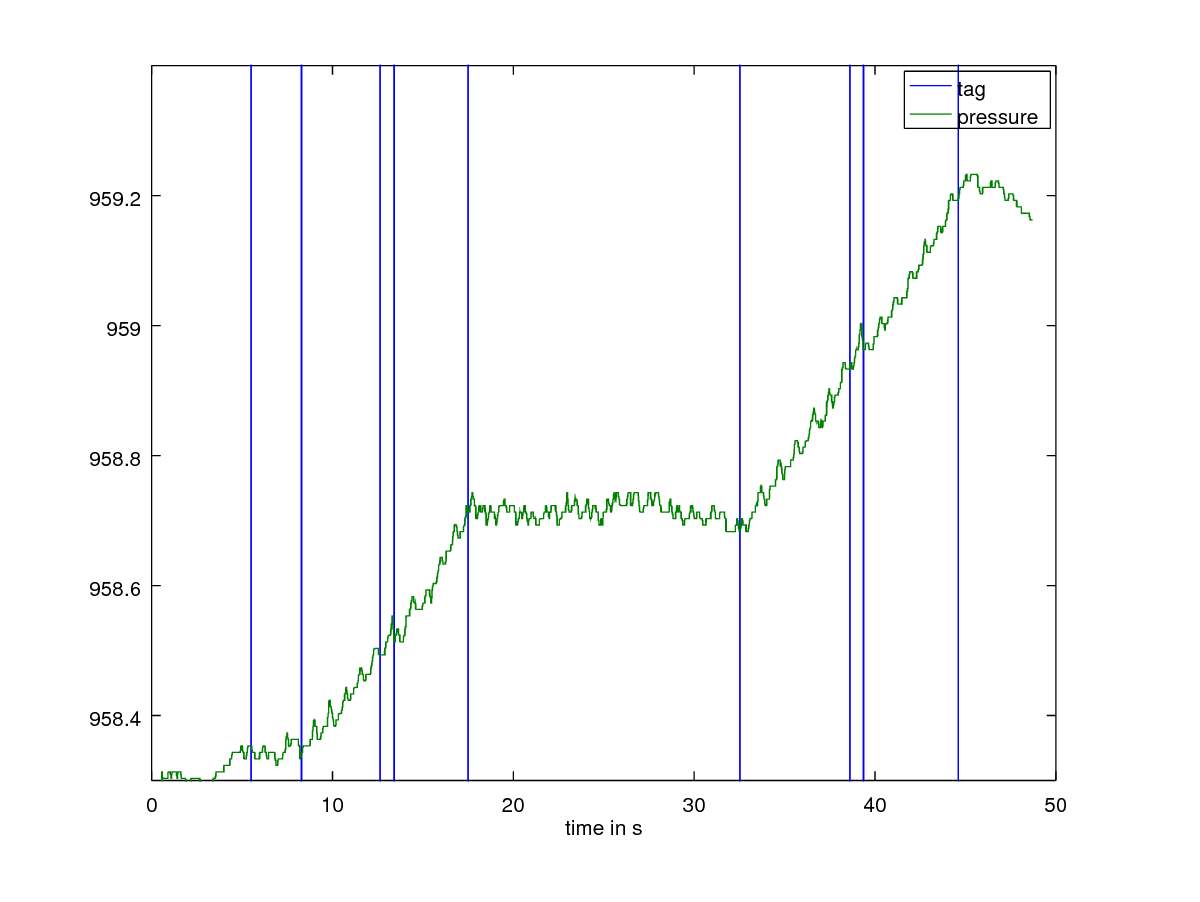
\includegraphics[width=.45\textwidth]{stairsfhdowna2_p} &
		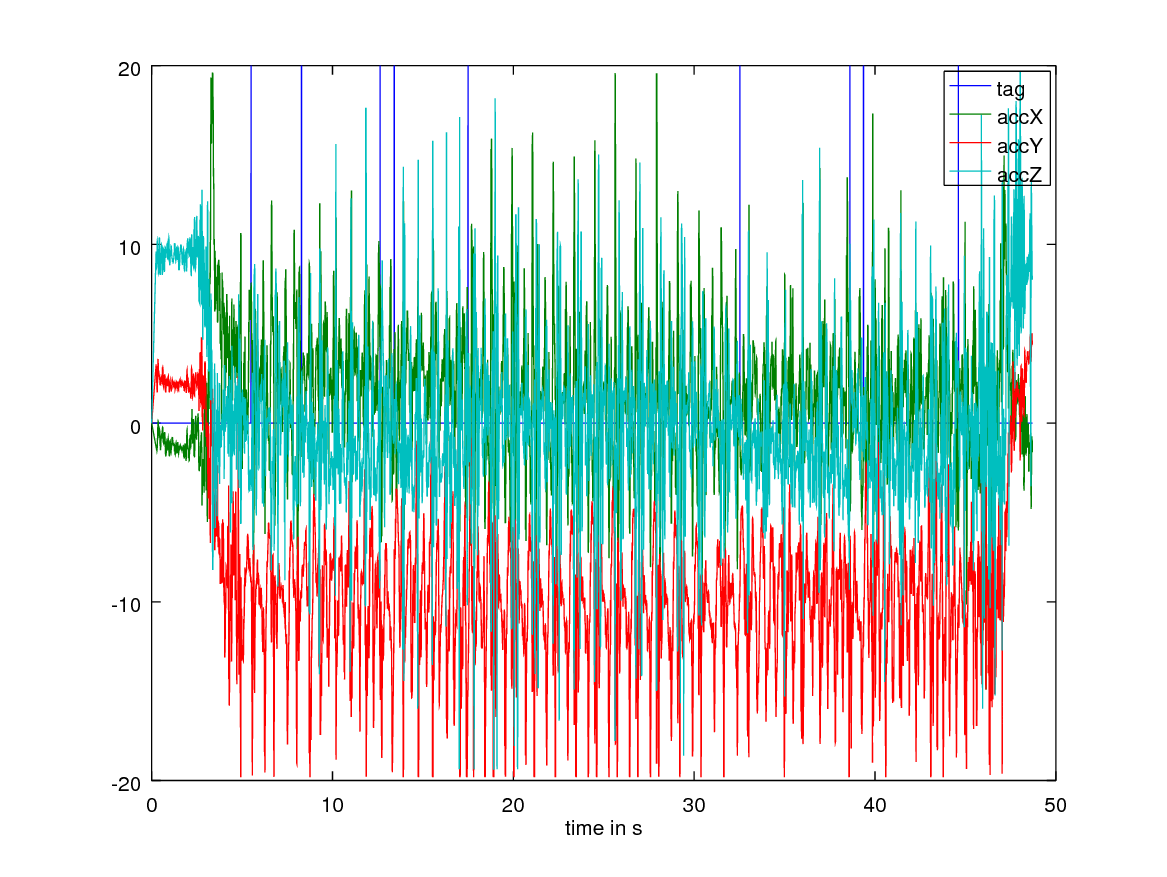
\includegraphics[width=.45\textwidth]{stairsfhdowna2_a} 
		\\
		(a) & (b)
		\\[4pt]	%vertical extra spacing (4 points)
		\includegraphics[width=.45\textwidth]{stairsfhdowna2_g} &
		\includegraphics[width=.45\textwidth]{stairsfhdowna2_la} 
		\\
		(c) & (d)
		\\[4pt]	%vertical extra spacing (4 points)
		\includegraphics[width=.45\textwidth]{stairsfhdowna2_atotal} &
		\includegraphics[width=.45\textwidth]{stairsfhdowna2_latotal} 
		\\
		(e) & (f)
	\end{tabular}
	%
	\caption{Test case 9}
	\label{fig:Test_case_stairs_9}
\end{figure}

%%%----------------------------------------------------------
\section{Test case 10}
%%%----------------------------------------------------------
Test case 10 in Fig.~\ref{fig:Test_case_stairs_10}
\begin{figure}
	\centering\small
	\setlength{\tabcolsep}{0mm}	% alle Spaltenränder auf 0mm
	\begin{tabular}{c@{\hspace{12mm}}c} % mittlerer Abstand = 12mm
		\includegraphics[width=.45\textwidth]{stairsfhdownf1_p} &
		\includegraphics[width=.45\textwidth]{stairsfhdownf1_a} 
		\\
		(a) & (b)
		\\[4pt]	%vertical extra spacing (4 points)
		\includegraphics[width=.45\textwidth]{stairsfhdownf1_g} &
		\includegraphics[width=.45\textwidth]{stairsfhdownf1_la} 
		\\
		(c) & (d)
		\\[4pt]	%vertical extra spacing (4 points)
		\includegraphics[width=.45\textwidth]{stairsfhdownf1_atotal} &
		\includegraphics[width=.45\textwidth]{stairsfhdownf1_latotal} 
		\\
		(e) & (f)
	\end{tabular}
	%
	\caption{Test case 10}
	\label{fig:Test_case_stairs_10}
\end{figure}